%------------------------------------------------
% Quick reference. 
%------------------------------------------------
%
% Для вставки картинок:
%
%--------         Комманда
%
%\begin{figure}[H]
%	\includegraphics{img_name}
%	\caption{some caption}
%	\label{some_pic}
%\end{figure}
%
%--------        Переменные
%
% img_name     <- Название картинки в папке img.
% some_caption <- подпись картинки.
% label        <- лейбл нужен для ссылок на картинку.
% H            <- расположение картинки на странице.
%
%--------         Пример
%
%\begin{figure}[H]
%	\includegraphics{pic1.jpg}
%	\caption{График зависимости какой-то}
%	\label{grapics1}
%\end{figure}
%
%------------------------------------------------
%
% Для референса по лейблу:
%
%--------         Комманда
%
% Для ссылки используется \eqref{ref}.
%
%--------        Переменные
%
% ref          <- указанный лейбл в директиве \label{ref}
%                 Ссылку можно сделать на любой объект имеющий \label{•}
%
%--------         Пример
%
% \eqref{graphics1}
%
%------------------------------------------------
%
% Для листинга кода:
%
%--------         Комманда
%
% \lstinputlisting[language=lang,mathescape=true]{src}
%--------        Переменные
%
% lang         <- язык на котором написан исходный код, например "python" или "C++".
% mathescape   <- если в исходниках есть формулы LaTeX, то они будут представлены как формулы.
% src          <- путь до файла исходников.
%
%--------         Пример
%
% \lstinputlisting[language=C++,mathescape=false]{./src/bullshit.cpp}
%
%------------------------------------------------
%
% Для вставки таблиц:
%
%--------
%\begin{table}[H]
%	\centering
%	\caption{ capt }
%	\begin{tabularx}{0.9\textwidth}{ | Y | Y | }
%		\hline
%		lines
%	\end{tabularx}
%	\label{tab1}
%\end{table}
%--------
% caption      <- Подпись таблицы.
% tab1         <- лейбл нужный для ссылки на таблицу.
% | Y | Y |    <- количество и формат столбцов.
% Y            <- Тип столбца.
%                 В данном случае определены кастомные столбцы Y (Спасибо Максиму Наумову)
% |            <- обозначает границы столбца.
%                 То есть, если будет указано |Y Y|, то столбцы внутри строк разделены не будут.
% H            <- То же самое, что и у картинок.
% lines        <- непосредственно элементы таблицы.
%                 Разделяются знаком "&", оканчивать каждую строку лучше \\ \hline
%
%--------         Пример
%\begin{table}[H]
%	\centering
%	\caption{ capt }
%	\begin{tabularx}{0.9\textwidth}{ | Y | Y | }
%		\hline
%		str1 & str2 \\ \hline
%		str1 & str2 \\ \hline
%		str1 & str2 \\ \hline
%		str1 & str2 \\ \hline
%		str1 & str2 \\ \hline
%	\end{tabularx}
%	\label{tab1}
%\end{table}
%------------------------------------------------

\documentclass[14pt, fleqn, a4paper]{extarticle}

\makeatletter
\renewcommand*\l@section{\@dottedtocline{1}{1.5em}{2.3em}}
\renewcommand*\l@subsection{\@dottedtocline{1}{3}{2.3em}}



%\includegraphics{universe}
\usepackage{titling}
\usepackage[utf8]{inputenc}
\usepackage[]{hyphenat}
\usepackage[T2A]{fontenc}
\usepackage[russian]{babel} % указывает язык документа
\usepackage[left=3cm,right=1.5cm,top=2cm,bottom=2.5cm,bindingoffset=0cm]{geometry}
\usepackage{lastpage}
\usepackage{fancyhdr}
\usepackage[compact]{titlesec}
\usepackage{graphicx} % для вставки картинок
\usepackage[intlimits]{mathtools} % математические дополнения
\usepackage{amssymb}
\usepackage[tableposition=top]{caption}
\usepackage{subcaption}
\usepackage{indentfirst}
\usepackage{pythonhighlight}
\usepackage{listings}
\usepackage{tabularx}
\usepackage{tabulary}
\usepackage{multirow}
\usepackage{float}
\usepackage[figure,table]{totalcount}
\usepackage{diagbox}
\usepackage[german=guillemets]{csquotes}
\usepackage{fontspec}
\usepackage[shortlabels]{enumitem}
%\usepackage{mathptmx}% http://ctan.org/pkg/mathptmx
%\usepackage{showframe}
\usepackage{hyperref}
\usepackage{siunitx}
\usepackage{ragged2e}

\setlength{\parindent}{1.2cm}

\setlength{\mathindent}{1.2cm}

\defaultfontfeatures{Ligatures={TeX},Renderer=Basic}
\setmainfont[Ligatures={TeX,Historic}]{Times New Roman}

%\setlist[enumerate]{itemindent=\dimexpr\labelwidth+\labelsep\relax,leftmargin=0pt}

%\setlength{\section*}{0.5cm}
%\usepackage{minted}
%\usepackage{fancyvrb}
%\usepackage{newtxtext}

%\titleformat{\section}[hang]{\bfseries\LARGE\centering}{}{1em}{}

%для нормального отображение списка источников и библиографических ссылок
\usepackage{ifthen}
\makeatletter
\renewcommand\@cite[2]{%
[#1] \hspace{-0.3cm} \ifthenelse{\boolean{@tempswa}}
{, \nolinebreak[3] #2 \hspace{-0.3cm}}{}
}
\newcommand\tab[1][1.25cm]{\hspace*{#1}}
\renewcommand\@biblabel[1]{ #1}
\makeatother

%\setlist[enumerate]{itemindent=\dimexpr\labelwidth+\labelsep\relax,leftmargin=0pt}
\setlist[enumerate,itemize]{leftmargin=0pt,itemindent=1.7cm, itemsep=-0.2cm, topsep =-0.2cm}
\titleformat{\section}{\bfseries\centering}{\thesection}{0.5em}{ \MakeUppercase }
%\titleformat{\subsection}{\large\bfseries\centering}{\thesubsection}{0.5em}{}
%\titleformat{\section}{\large\bfseries\centering}{\thesection}{0.5em}{\MakeUppercase}
\titleformat{\subsection}[block]{\sloppy \bfseries  \hspace{1.2cm}}{\thesubsection}{0.5em}{\vspace{-0.2cm}}
%\setlength{\subsection*}{1.5cm}
%\setlength{\parindent}{4em}

%\setlength{\parindent}{1.5cm}

\usepackage{tocloft}
\usepackage{amsmath}

\renewcommand{\cftdotsep}{1} % Set dots at each "pixel"(?)

\renewcommand{\cfttoctitlefont}{\normalfont\hfill\bfseries\MakeUppercase} % Format toc title
\renewcommand{\cftaftertoctitle}{\hfill}                                  % to look good

\setlength{\cftbeforesecskip}{0pt} % Remove skip before section title

\renewcommand{\cftsecfont}{\normalfont} % Set section title font to normal
\renewcommand{\cftsecpagefont}{\normalfont} % Set section page font to normal

\renewcommand{\cftsecleader}{\cftdotfill{\cftdotsep}} % Add dots to section titles

\setlength{\cftsecindent}{0cm}% Set indent for \section
\setlength{\cftsubsecindent}{1cm}% Set indent for \subsection

\captionsetup[figure]{name={Рисунок},labelsep=endash, skip=5pt}
\setlength{\belowcaptionskip}{-1cm}
\captionsetup[table]{name={Таблица},labelsep=endash,singlelinecheck=false, skip=5pt, margin=1cm, justification = raggedright}


%\renewcommand{\baselinestretch}{1.5}
\linespread{1.5} % полуторный интервал
\frenchspacing
\graphicspath{ {images/} }

%-------------------------------------------
% Переменные
%-------------------------------------------

\newcommand{\firstAuthorSurName}{Наумов}                                               % Фамилия автора.
\newcommand{\firstAuthorInitials}{ М. Е.}                                               % Фамилия автора.
\newcommand{\leftcolon}{Уравнения Математической Физики}
\newcommand{\secondAuthorSurName}{Родин}                                               % Фамилия автора.
\newcommand{\secondAuthorInitials}{ И. А.}                                               % Фамилия автора.
\newcommand{\teacherName}{Дегтярев А. А.}                                               % Имя преподавателя.
\newcommand{\variantNumber}{25}                                                       % Номер варианта.
\newcommand{\groupNumber}{6409-010302D}                                               % Номер группы.
\newcommand{\subjectTitle}{Отчет о научно-исслдеовательнсокй работе бакалавра}                                  % Название предмета.
\newcommand{\taskTitle}{Дисциплина \enquote{Численные методы математической физики}}          % Название работы.
\newcommand{\theme}{РЕШЕНИЕ ЗАДАЧ МАТЕМАТИЧЕСКЙ ФИЗИКИ МЕТОДОМ КОНЕЧНЫХ РАЗНОСТЕЙ}          % Название работы.

%-------------------------------------------
% Ссылки в оглавлении
%-------------------------------------------


\hypersetup{
colorlinks,
citecolor=black,
filecolor=black,
linkcolor=black,
urlcolor=black
}

%-------------------------------------------
% Стиль футеров и хедеров
%-------------------------------------------

\pagestyle{fancy}
\fancyhead[L, R]{}
\fancyfoot[L]{}
\fancyfoot[R]{}
\renewcommand{\footrulewidth}{0pt}
\renewcommand{\headrulewidth}{0pt}
\captionsetup{justification = centering,
singlelinecheck = false}

%\renewcommand\subsectionfont{\normalfont\normalsize\bfseries}



% Для листинга

\lstset{
basicstyle=\footnotesize\ttfamily,
columns=fullflexible,
keywordstyle=\color{blue},
%frame=single,
breaklines=true,
numberstyle=\tiny\color{mygray},
postbreak=\mbox{\textcolor{red}{$\hookrightarrow$}\space},
showstringspaces=false,
}

\newcolumntype{Y}{>{\centering\arraybackslash}X}

\begin{document}

    %----------------------------------------------------------------------------------------
    %	TITLE PAGE
    %----------------------------------------------------------------------------------------
    \pagenumbering{Alph}

    \begin{titlepage}

        \center

        %------------------------------------------------
        %	Заголовки
        %------------------------------------------------

        {МИНИСТЕРСТВО НАУКИ И ВЫСШЕГО ОБРАЗОВАНИЯ РОССИЙСКОЙ ФЕДЕРАЦИИ\\
        {Федеральное государственное автономное  \\[-0.2cm]
        образовательноеучреждение высшего образования\\[-0.2cm]
        «Самарский национальный исследовательский университет \\[-0.2cm]
        имени академика С.П.Королёва»\\[-0.2cm]
        (Самарский университет)}\\[0.7cm]
        {Институт информатики, математики и электроники}\\[-0.2cm]
        {Факультет информатики}\\[-0.2cm]
        {Кафедра технической кибернетики}\\[2cm]
        }

        %------------------------------------------------
        %	Название работы
        %------------------------------------------------

        \vfill\vfill


        \vfill

        \begin{center}
            ВЫПУСКНАЯ КВАЛИФИКАЦИОННАЯ РАБОТА \\[1cm]
            \textbf{\large Моделирование и исследование распространения пучков Эйри и Пирси} \\[1cm]
            по направлению подготовки\\[-0.2cm]
            01.03.02 Прикладная математика и информатика (уровень бакалавриата)\\[2cm]
        \end{center}

        \begin{minipage}{0.8\textwidth}
            Студент    \hfill    И.А. Родин \\
            Руководитель ВКР, к.ф.-м.н., доцент \hfill  С.А. Дегтярев\\
            Нормоконтролёр        \hfill С.В. Суханов\\
        \end{minipage}

        \vfill\vfill\vfill

        {\centering Самара \the\year}


    \end{titlepage}

    \pagenumbering{arabic}

    \setcounter{page}{2}


    %------------------------------------------------
    %Задание
    %------------------------------------------------



    %------------------------------------------------
    % Реферат
    %------------------------------------------------

    \section*{ЗАДАНИЕ}{

    \center
    {фывфывМИНИСТЕРСТВО НАУКИ И ВЫСШЕГО ОБРАЗОВАНИЯ РОССИЙСКОЙ ФЕДЕРАЦИИ\\
    {Федеральное государственное автономное  \\[-0.2cm]
    образовательноеучреждение высшего образования\\[-0.2cm]
    «Самарский национальный исследовательский университет \\[-0.2cm]
    имени академика С.П.Королёва»\\[-0.2cm]
    (Самарский университет)}\\[1cm]
    {Институт информатики, математики и электроники}\\[-0.2cm]
    {Факультет информатики}\\[-0.2cm]
    {Кафедра технической кибернетики}\\[1cm]
    }

    \makebox[\textwidth][r]{% create a box, with it's content aligned to the right
    \begin{minipage}{.5\textwidth}% create a content half width
        \begin{center}
            УТВЕРЖДАЮ\\[-0.2cm]
            Заведующий кафедрой  \\[-0.6cm]
        \end{center}
        \begin{flushright}
        { \rule{115 pt }{1 pt}А.В. Куприянов }
            \\
            { ''    \rule{20 pt }{1 pt}  ''  \rule{100 pt }{1 pt} 20    \rule{20 pt }{1 pt} г. }
        \end{flushright}
    \end{minipage}
    }

    }
    \newpage
    \section*{РЕФЕРАТ}
    {
    \textbf{Выпускная квалификационная работа бакалавра:}
    \pageref{LastPage} страниц,
    \totalfigures\ рисунков,
    14 источника,
    1 приложение.

    \textbf{Презентация:} n слайдов.

    \textit{ПУЧКИ ЭЙРИ, ПУЧКИ ПИРСИ, БЕЗДИФРАКЦИОННЫЕ ПУЧКИ, ПРЕОБРАЗОВАНИЕ ФУРЬЕ, ПРЕОБРАЗОВАНИЕ ФРЕНЕЛЯ, УСКОРЯЮЩИЕСЯ ПУЧКИ, ЧИСЛЕННОЕ
    ИНТЕГРИРОВАНИЕ}

    Объектом исследования данной научно-исследовательской работы
    являются бездифракционные пучки Эйри и Пирси, представленные в данном
    исследовании в виде комплексной функции действительных переменных.

    Целью данной научно-исследовательской работы является построение и
    рассмотрение пучков, их свойств, а также результата применения к данным пучкам различных операторов распространения.

    Разработана программа, осуществляющая построение
    рассмотренных пучков, вычисление необходимых характеристик, численное
    преобразование Френеля, двумерное и одномерное преобразования Фурье на произвольных участках рассмотрения. Был
    произведен анализ влияния параметров моделирования на выходной результат.


    }
    \newpage

    \newpage
    \tableofcontents
    \newpage

    %------------------------------------------------
    % Введение
    %------------------------------------------------

    \section*{Введение}
    {
    \addcontentsline{toc}{section}{Введение}

    В рамках данной научно-исследовательской работы рассматриваются и
    моделируются несколько разновидностей бездифракционных пучков, а именно
    пучки Эйри и Пирси. Эти пучки обладают рядом уникальных свойств, которые являются причиной большого интереса со стороны современного научного сообщества.
    Среди важных свойств пучков Эйри можно озвучить следующие [\ref{first_airy},~\ref{airy_wiki}]:
    \begin{itemize}
        \item[$-$] ускорение;
        \item[$-$] самофокусировка;
        \item[$-$] бездифракционность;
        \item[$-$] самовосстановление.
    \end{itemize}
    \vspace{0.2cm}
    Остановимся на каждом из свойств подробнее.

    Данные пучки являются ускоряющимися, то есть распространяются по некоторой криволинейной траектории, зависящей от определенных параметров.
    Благодаря данному свойству могут быть достигнуты области пространства, скрытые от прямого наблюдения.

    Второе свойство пучков вызывает, пожалуй, наибольший интерес, так как открывает возможность использования данных пучков в мире микромеханики и,
    в частности, в сфере различных микроманипуляций. Суть свойства заключается в том, что если расположить в пространстве несколько источников излучения,
    то благодаря свойству ускорения в определенной точке такая оптическая установка создаст фокус -- некоторую область пространства,
    при попадании частиц в которую эти частицы будут там удерживаться и перемещаться вслед за этой областью.
    Экспериментальная реализация данного подхода уже была продемонстрирована на примере перемещения частиц через препятствие.

    Третье свойство представляет существенный интерес для современной оптики, потому что пучки Эйри не изменяют своего вида при распространении.
    Однако здесь стоит заметить, что данное утверждение справедливо для математической модели, бесконечной абстракции,
    когда входное распределение берется определенным на протяжении всей вещественной оси. На практике, к сожалению,
    такого результата добиться невозможно, поскольку для возможности моделирования распространения различных пучков их начальное
    распределение урезается до какого-то конечного отрезка рассмотрения. В этом случае свойства неподверженности дифракции все же сохраняется,
    однако только при распространении на конечные расстояния. В теории данное свойство может быть использовано для передачи информации,
    поскольку если гарантируется, что внешний вид сигнала не изменился, то после его приема можно точно установить параметры
    сигнала в точке отправления и таким образом передать информацию. Однако для реализации данной технологии еще предстоит решить перечень определенных проблем.

    Последнее свойство пучков заключается в их способности восстаналивать свой общий вид после определенного времени расространения при встрече некоторого препятствия на своем пути.

    Вид этих пучков берет свое начало в теории катастроф~[\ref{catastrophe}]. Свое название пучки Эйри получили от интеграла Эйри, который был
    получен Джорджем Эйри для объяснения оптических каустик, таких как те, что
    проявляются в виде радуги~[\ref{Khonina_2008}]. Воспроизвести и пронаблюдать пучки Эйри
    впервые удалось ученым из Флориды в 2007 году~[\ref{first_airy},~\ref{Khonina_2008}].

    Пучки Пирси также
    получили свое название от одноименного интеграла, который часто
    применяется для решения проблем распространения волн и дифракции~[\ref{pe_selfheal}] \hspace{-0.3cm}. Несмотря на то,
    что некоторыми из перечисленных выше свойств пучки Пирси не обладают, например, свойством ускорения,
    существует возможность с помощью нехитрых манипуляций привести их к виду, сильно напоминающему по внешнему виду и свойствам пучки Эйри.
    Аналогичные рассуждения справедливы и для пучков Эйри.

    В рамках данной работы реализована программа,
    осуществляющая построение пространственных пучков Эйри и Пирси в качестве исследовательской составляющей, а так же
    программный модуль, позволяющий промоделировать формирование
    данных пучков при прохождении через линзу с различными физическими характеристиками и распространение на свободное расстояние как с использованием,
    так и без использования оптических элементов.
    Среди параметров, рассматриваемых в данной работе, будут изучены
    амплитуда, фаза и вещественная и мнимая части выходного поля.


    }
    \newpage

    %------------------------------------------------
    % Начало основной части
    %------------------------------------------------

    \titleformat{\section}[block]
    {\sloppy \bfseries}
    {\hspace{1.2cm}\thesection}
    {1ex}{}
    \titlespacing*{\section}{0pt}{1ex}{1em} %!!!!!!!!!!!!!!!!!!!!!!!!!!!!!!!!!!!!!!!!!!!!!!!!!!!!!!!!!!!!!!!!!!!!!!!!!!!!!!!!!!!!!
    %\titleformat{\section}{  \sloppy  \bfseries   }{ \thesection}{1ex}{}
    %\titlespacing*{\section}{\parindent}{1ex}{1em}
    %\titlespacing*{\subsection}{0pt}{4em}{3em}
    \section{Обзор теоретических основ для ускоряющихся пучков}
    {
    Уравнение, описывающее пучки Эйри, является аналитическим решением
    следующего дифференциального уравнения:
    \begin{equation*}
        \label{1}
        \frac{\partial^2 \omega}{\partial z^2} = z \omega,
    \end{equation*}
    и выглядит следующим образом:
    \begin{equation}
        \label{2}
        \frac{1 }{2 \pi}\int_{- \infty}^{\infty} exp[{\frac{i\alpha t^3}{3} + ixt}]dt,
    \end{equation}
    что является известным результатом~[\ref{Khonina_2011}, ~\ref{math_func}].
    Принимая во внимание формулу одномерного обратного преобразования Фурье, имеющую следующий вид [\ref{zorich}]:
    \begin{equation}
        \label{100}
        \frac{1 }{2 \pi}\int_{- \infty}^{\infty} f(x)exp[ixt]dt,
    \end{equation}
    нетрудно заметить, что равенство~\eqref{100} также является
    преобразованием Фурье от функции:
    \begin{equation}
        \label{airy_eq}
        F(t) = exp[\frac{i \alpha t^3}{3}],
    \end{equation}
    которая в дальнейшем будет рассматриваться в качестве входного поля в виде пространственного спектра
    рамках исследования.

    Уравнение, описывающее пучки Пирси, задается интегралом Пирси:
    \begin{equation*}
        \label{4}
        Pe(x, y)  = \int_{-\infty}^{\infty}exp[i(t^4 + xt^2 +yt)]dt,
    \end{equation*}
    что тоже в свою очередь является обратным преобразованием Фурье от функции
    следующего вида:
    \begin{equation*}
        \label{5}
        F(x, t)  = exp[i(t^4 + xt^2)],
    \end{equation*}
    которая будет рассматриваться как входное поле при моделировании пучков
    Пирси~[\ref{pe_art}].

    Для численного интегрирования было принято решение использовать стандартную формулу
    прямоугольников, так как она представляется наиболее простой в реализации и
    имеет наибольшую точность среди всех способов численного интегрирования
    нулевого порядка. В классическом варианте формула выглядит следующим
    образом~[\ref{samarsky}]:
    \begin{equation}
        \label{integration}
        \int_a^b{f(x)dx} \approx \sum_{i=0}^{n-1} f(\frac{x_{i+1} + x_i}{2})(x_{i+1} - x_i),
    \end{equation}
    однако в рамках данной работы исходная функция является функцией двух аргументов,
    поэтому результатом такого численного интегрирования станет значение
    выходной функции в конкретной точке, то есть:
    \begin{equation*}
        \label{7}
        f(u_j) \approx \sum_{i=0}^{n-1}f(\frac{x_{i+1}+x_i}{2})(x_{i+1} - x_i) exp[i \frac{k}{f}(\frac{x_{i+1}+x_i}{2})u_j].
    \end{equation*}

    Однако не всегда научный интерес может ограничиться информацией, получаемой из одномерного преобразования Фурье.
    Во многих случаях значительно нагляднее продемонстрировать результат моделирования в виде поверхности.
    Для достижения данного результата используется двумерное преобразование Фурье, которое имеет следующий вид [\ref{zorich}]:
    \begin{equation}
        \label{2d_four}
        G(u, v) = \frac{k}{f}\int_{-\infty}^{+\infty} \int f(x, y)exp[\frac{-ik}{f}(xu+yv)] dxdy,
    \end{equation}
    \tab    где $x, y$ -- пространственные переменные входного поля;  \\
    \tab \tab \hspace{-0.4cm}$u, v$ -- пространственные переменные выходного поля;\\
     \tab \tab \hspace{-0.4cm} $k$ -- волновое число;\\
    \tab \tab \hspace{-0.4cm} $f$ -- фокусное расстояние.

    В данной работе двойное интегрирование в формуле тоже было заменено численным аналогом.

    Кроме того, определенный интерес в рамках данного исследования может представлять реализация преобразования Френеля,
    физический смысл которого заключается в распространении пучка на некоторое расстояние $z$. Общий вид одномерного преобразования Френеля [\ref{fres}]:
    \begin{equation}
        \label{fresnel}
        F(u) = - \sqrt{\frac{ik}{2 \pi z}}exp[{ikz}]\int_{-\infty}^{+\infty}f(x) exp[{\frac{ik}{2z}(x - u)^2}],
    \end{equation}
    \tab где $z $-- расстояние распространения.\\
    Кроме того, множество случаев, для которых допустимо использовать данную формулу, ограничивается условием $x-u\ll z$.

    Стоит отметить, что преобразование Фурье моделирует распространение в ситуации,
    когда начальная и конечная плоскости рассмотрения являются фокальными плоскостями линзы.
    Данное ограничение не всегда удовлетворяет интерес исследований,
    поэтому в рамках этой научной работы было принято решение совместить преобразование Френеля и Фурье,
    чтобы иметь возможность рассмотреть выходное распределение на некотором произвольном расстоянии от выходной фокальной плоскости линзы.
    Достичь подобного результата можно за счет включения в оператор распространения на свободное расстояние оптического элемента.
    В математическом смысле это значит, что преобразование Френеля умножается на экспоненту определенного вида.
    В данном случае воспользуемся следующей реализацией:
    \begin{equation*}
        exp[-ik \frac{x^2}{2f} ].
    \end{equation*}

    Тогда раскроем квадрат в показателе экспоненты, вынесем за знак интеграла слагаемое, содержащее $u^2$,
    так как оно не зависит от переменной интегрирования, и внесем добавленный оптический элемент под знак интеграла.
    После группировки некоторых слагаемых получим:
    \begin{equation*}
        F(u) = - \sqrt{\frac{ik}{2 \pi z}}exp[ikz] exp[{ \frac{iku^2}{2z} }] \int_{-\infty}^{+\infty}f(x) exp[\frac{ikx^2}{2}( \frac{1}{z} - \frac{1}{f})] exp[{ik \frac{ux}{z}}]dx,
    \end{equation*}
    \tab    где $f$ -- фокусное расстояние линзы;\\
    \tab \tab \hspace{-0.4cm}$z$ -- расстояние от начальной плоскости до линзы.
    }\label{sec:обзор-теоретических-основ-для-ускоряющихся-пучков}
    \newpage

    \section[Описание программной реализации пучков и операторов распространения]{\nohyphens{Описание программной реализации пучков и операторов распространения}}
    {
    Для написания программы использовался язык
    программирования Python, так как он позволяет легко реализовать весь
    необходимый функционал, предлагает большой выбор готовых средств для
    использования, сравнения и проверки результатов. Работа велась в среде
    разработки JetBrains PyCharm, поскольку она удобна и предоставляет
    множество возможностей, существенно упрощающих и ускоряющих написание
    исходного кода.

    Одним из вариантов решения поставленной задачи является использование готовой библиотеки для
    быстрого преобразования Фурье. Подобный функционал предоставляют
    различные библиотеки, в рамках данной работы были использованы
    библиотеки Numpy и Scipy~[\ref{np}]. Однако область их применения в рамках
    дискретного преобразования Фурье ограничена теми случаями, когда массивы
    аргументов для входной и выходной функции одинаковы.
    Это ограничение противоречит целям, преследуемым в данной работе, поэтому после получения
    первых результатов было принято решение отказаться от использования
    данного программного обеспечения и реализовать собственный модуль
    численного интегрирования методом прямоугольников, реализующий
    преобразование Фурье на произвольных массивах аргументов.

    Спецификой рассматриваемых пучков является факт того, что функции,
    описывающие их – комплексные экспоненты, поэтому при работе и детальном
    рассмотрении полученных результатов не обойтись без работы с функциями,
    которые позволяют получить некоторые характеристики из массива
    комплексных чисел. В данной работе подобными функциями являются
    функция взятия модуля комплексного числа, функция взятия фазы
    комплексного числа, а также функции взятия действительной и мнимой части.
    Кроме того, требовалась программная реализация экспоненциальной функции,
    которая корректно работала с комплекснозначными аргументами.
    Такой функционал предоставляет библиотека cmath~[\ref{cmath}] и Numpy.
    В ходе написания программы было выяснено, что библиотека cmath работает в разы медленнее,
     чем аналогичный функционал из библиотеки Numpy, поэтому выбор был сделан в пользу последней.


    В качестве численного метода интегрирования был выбран метод
    центральных прямоугольников, потому что он наиболее прост в реализации и
    предоставляет наибольшую точность среди всех методов нулевого порядка.
    Кроме того, особенности рассматриваемых пучков, а именно наличие быстро осциллирующих составляющих,
    позволяет использовать метод прямоугольников практически без потери точности относительно, например, метода Симпсона.
    Отказ от использования готовых реализаций численного интегрирования связан
    с трудностями с параметризацией и общим сложным видом интегрируемых
    функций, рассматриваемых в работе.

    Для визуализации результатов использовался модуль Matplotlib~[\ref{plt}],
    так как он наиболее прост в использовании и предоставляет весь
    необходимый функционал для задач, поставленных в рамках данной научноисследовательской работы.

    \sloppy{
    На рисунках~\ref{pycharm} и~\ref{matplotlib} представлен внешний вид среды разработки Pycharm и
    пользовательский интерфейс взаимодействия с графиками библиотеки
    Matplotlib.
    }
    \begin{figure}[H]
        \begin{center}
            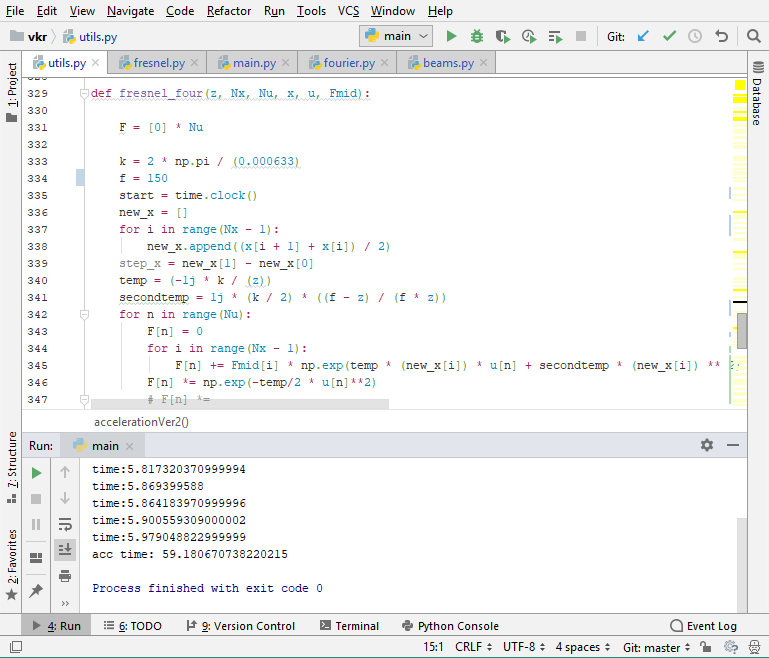
\includegraphics[width=10cm]{plots/pycharm1}
            \vspace{0.4cm}
            \caption{Внешний вид среды разработки PyCharm}
            \label{pycharm}
        \end{center}
    \end{figure}

    \vspace{0.1cm}

    \begin{figure}[H]
        \begin{center}
            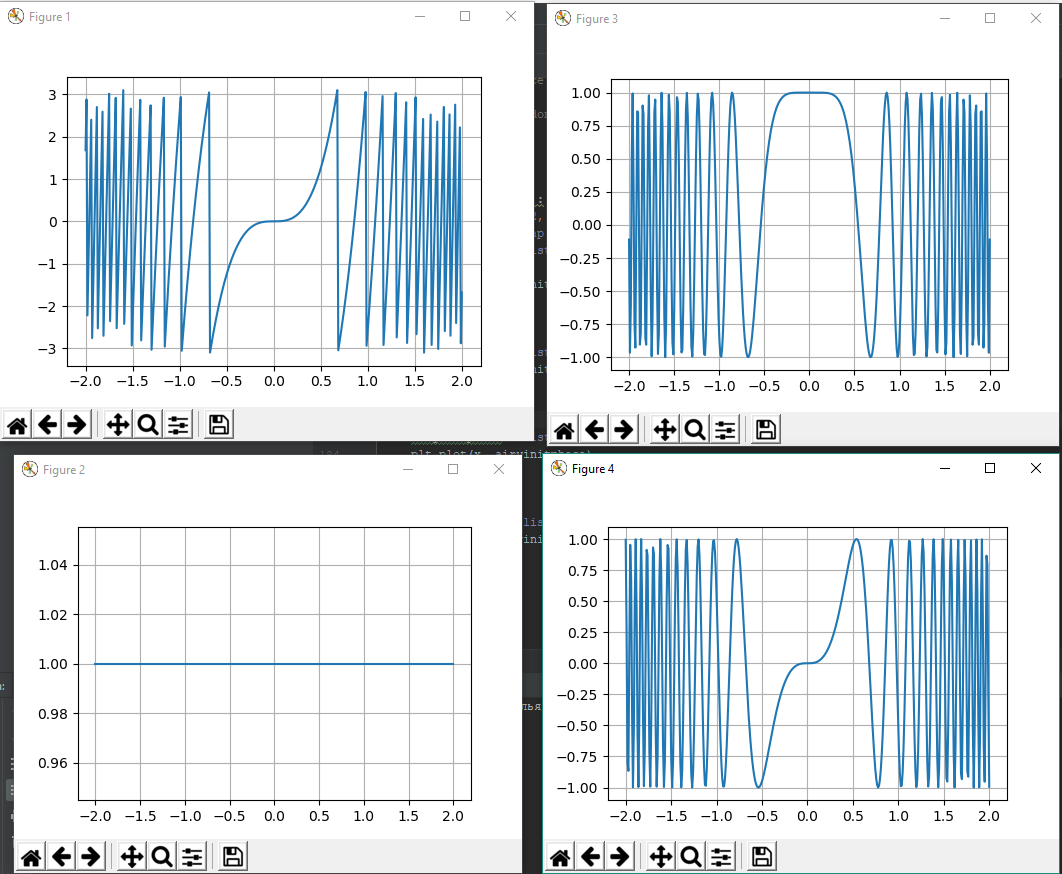
\includegraphics[width=10cm]{plots/matplotlib}
            \vspace{0.4cm}
            \caption{ Интерфейс взаимодействия с графиками, предоставляемый билиотекой Matplotlib}
            \label{matplotlib}
        \end{center}
    \end{figure}
    }\label{sec:nohyphens3}

    \newpage
    %\captionsetup[figure]{name={Рисунок},labelsep=endash, skip=5pt}


    \section[Построение входных распределений пучков Эйри, Пирси и их модификаций в виде пространственных спектров]{\nohyphens{Построение входных распределений пучков Эйри, Пирси и их модификаций в виде пространственных спектров}}{

    \subsection[Численное моделирование входного распределения пучков Эйри]{\nohyphens{Численное моделирование входного распределения пучков Эйри}}
    Входное поле для пучков Эйри имеет вид \eqref{airy_eq}.

    Исходя из вида комплексной функции, нетрудно заметить, что амплитуда
    входного поля для любого аргумента будет равна 1. В свою очередь фазой
    входного поля будет является кубическая парабола, однако поскольку фаза
    комплексного числа изменяется в пределах от -π до π или от 0 до 2π , то концы
    этой параболы будут представлять из себя набор сгущающихся линий по краям
    картинки.

    Кроме того, рассматриваемая функция имеет параметр-множитель у
    кубического члена показателя экспоненты. Варьируя этот параметр, можно
    получить различную фазу входного поля, что в дальнейшем может
    существенно сказаться на амплитуде и фазе выходного поля~[\ref{Khonina_2011}]. В остальном
    представление данной функции в виде стандартной функции языка
    программирования Python полностью удовлетворяет требованиям, которые
    накладывает общий подход к реализации программного комплекса.
    Поскольку объем данных, которые подаются на вход преобразованию
    Фурье сильно влияет на качество выходных данных, то будет рационально
    увеличивать коэффициент перед кубическим слагаемым, так как таким образом
    увеличивается объем полезных данных на той же длине рассматриваемого
    отрезка, то есть можно получить более качественный результат за то же время
    моделирования. Результаты моделирования для различных значений параметра представлены на рисунках~\ref{airy_phase} и~\ref{airyphase1}.
    \begin{figure}[H]
        \begin{center}
            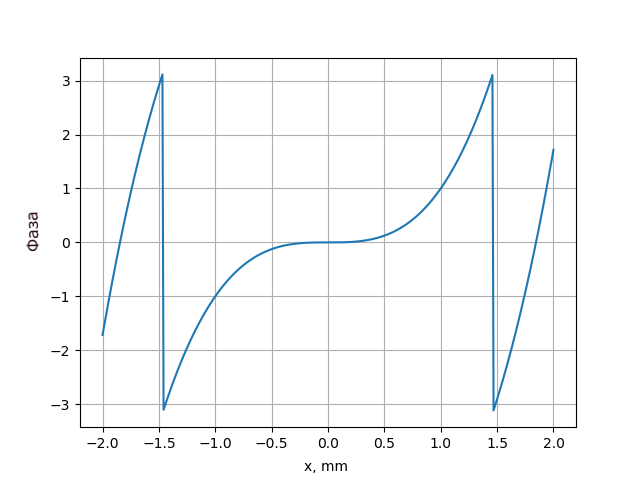
\includegraphics[width=10cm]{plots/airyphase}
            \caption{Фаза входного поля Эйри при $\alpha  = 1$}
            \label{airy_phase}
        \end{center}
    \end{figure}

    \begin{figure}[H]
        \begin{center}
            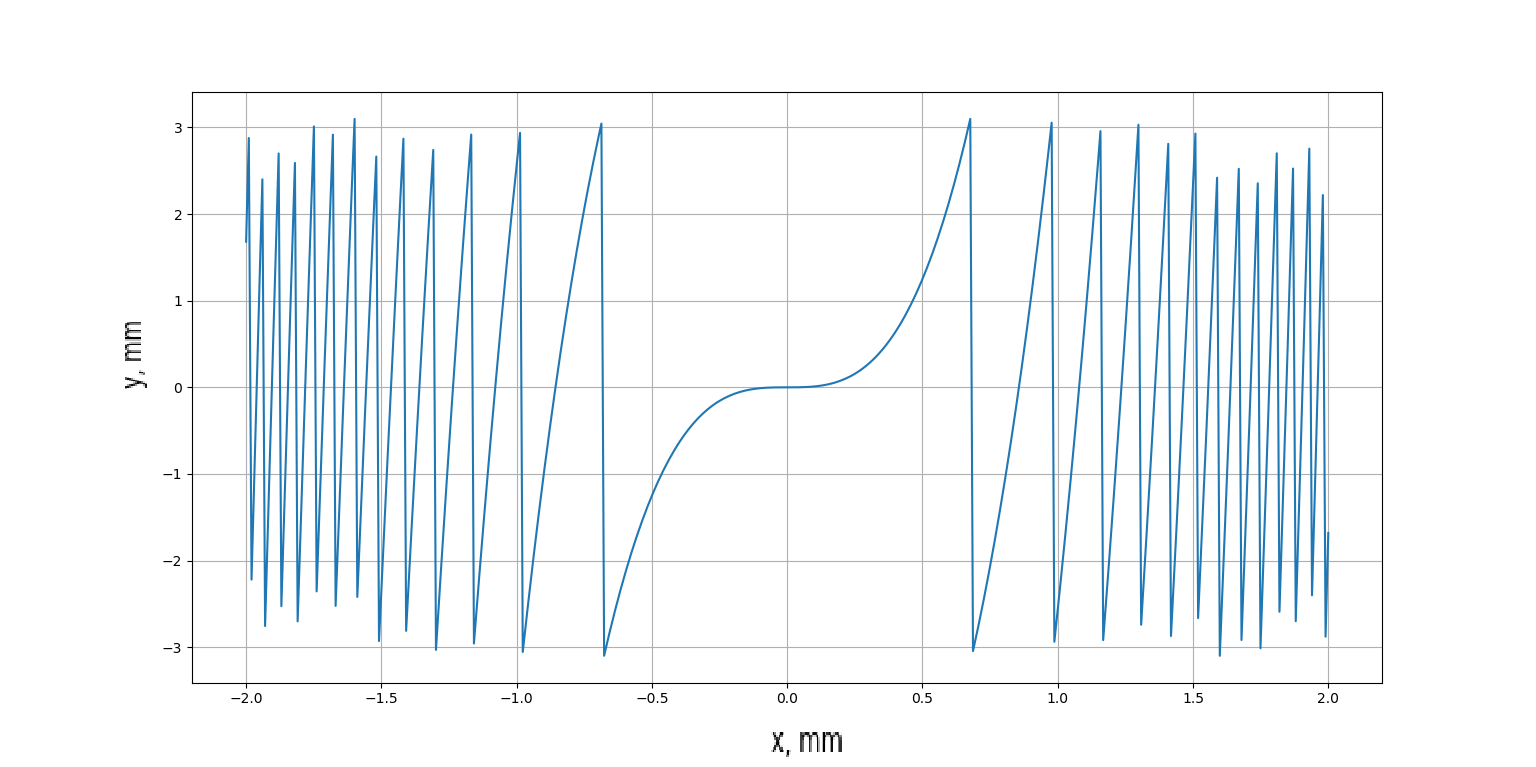
\includegraphics[width=10cm]{plots/airyphase1}
            \caption{  Фаза входного поля Эйри при $\alpha  = 30$}
            \label{airyphase1}
        \end{center}

    \end{figure}

    Сравнивая данные изображения, нетрудно заметить, что с увеличением
    параметра значительно увеличивается объем информации на одном и том же
    рассматриваемом отрезке. Этим приемом можно воспользоваться в
    дальнейшем, чтобы получить более информативное изображение выходного поля без увеличения времени вычислений, возникающего вследствие
    увеличения исследуемого отрезка.

    Аналогичным образом можно получить двумерную картину фазы начального распределения пучков,
    которая в дальнейшем будет использоваться в качестве входных данных для двумерного преобразования Фурье.
    Вид двумерного пучка Эйри:
    \begin{equation*}
        \label{zero_time_condition}
        f(x, y) = exp(\frac{i \alpha x^3 + i \alpha y^3}{3}).
    \end{equation*}
    Двумерная фаза входного распределния представлена на рисунке~\ref{airy_phase_2d}.

    \begin{figure}[H]
        \begin{center}
            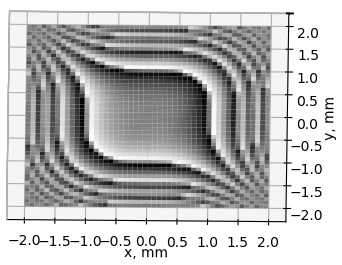
\includegraphics[width=10cm]{plots/airy_phase_2d_ortho}
            \caption{Двумерная фаза входного поля Эйри при $\alpha  = 3$}
            \label{airy_phase_2d}
        \end{center}

    \end{figure}

    Программная реализация входного поля пучков Эйри и графической
    интерпретации его амплитуды, фазы, действительной и мнимой части
    приведена в разделе 1 приложения А.


    \subsection{Численное моделирование входного распределения пучков Пирси}
    {
    Общий вид моделируемого входного поля для пучков Пирси может быть
    представлен следующим образом:
    \begin{equation*}
        f(x, t)  = exp[i(x^4 + tx^2)].
    \end{equation*}

    \sloppy{По аналогии с входным полем для пучков Эйри, помимо основного
    аргумента $x$ в функции присутствует параметр, варьируя который можно
    изменять фазу входного поля и изменять характеристики выходного поля.
    Амплитуда входного поля также равна 1. Существенным различием между
    этими двумя функциями является то, что фаза входного поля пучков Эйри
    представляет собой нечетную функцию, в то время как фаза входного поля
    пучков Пирси, представленная на рисунке~\ref{pearceyphase} – функция четная, что окажет
    определенное влияние на внешний вид выходных полей рассматриваемых
    пучков. Для пространственного спектра пучков Пирси просто получить двумерную картину, так как она
    получается декартовым произведением массивов значений выходной функции
    по осям $OX$ и $OY$, которые идентичны. На рисунке~\ref{pearceyphase} представлена фаза входного поля Пирси.}

    \begin{figure}[H]
        \begin{center}
            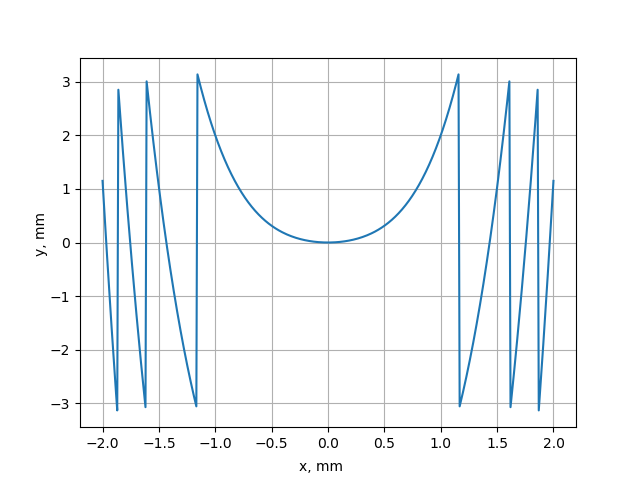
\includegraphics[width=10cm]{plots/pearceyphase}
            \caption{Фаза входного поля Пирси $\alpha  = 1$}
            \label{pearceyphase}
        \end{center}
    \end{figure}

    Схожим образом получается двумерный вид пучка:
    \begin{equation*}
        f(x, y)  = \exp(i(x^4 + y^4 + tx^2 + ty^2))
    \end{equation*}
    и двумерная фаза входного распределения, представленная на рисунке~\ref{pearcey_phase_2d}.
    \begin{figure}[H]
        \begin{center}
            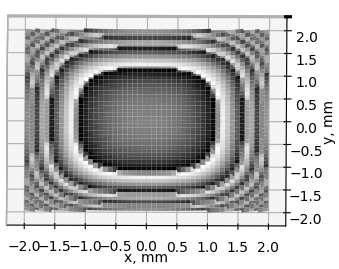
\includegraphics[width=10cm]{plots/pearcey_phase_2d_ortho}
            \caption{Двумерная фаза входного поля Пирси при $\alpha  = 1$}
            \label{pearcey_phase_2d}
        \end{center}
    \end{figure}

    Программная реализация входного поля пучков Пирси и графической
    интерпретации его амплитуды, фазы, действительной и мнимой части
    приведена в разделе 1 приложения А.
    }\label{subsec:численное-моделирование-входного-распределения-пучков-пирси}

    \subsection{Изменение характеристик пространственных спектров}{
    Нетрудно заметить, что основное отличие между описанными выше пучками заключается в виде функции в показателе экспоненты.
    Это базовое отличие определяет некоторые свойства пучков, например, нечетность функции делает пучок ускоряющимся,
    а четность влечет за собой обратный эффект. Однако в некоторых ситуациях проще модифицировать существующих пучок,
    нежели создавать новый, поэтому произведение над пучками подобных преобразований представляет определенный научный интерес.

    Для пучков Эйри задача заключается в модификации функции в показателе экспоненты с целью добиться ее четности.
    Наиболее простая реализация данной задачи заключается в добавлении модуля к аргументу функции.
    В таком случае входная функция примет следующий вид:
    \begin{equation*}
        AiEven(x) = exp[-it \frac{|x|^3}{3}].
    \end{equation*}
    Поскольку амплитуда входного поля по-прежнему остается единицей, обратим внимание на график фазы входной функции,
    вид которой представлен на рисунке~\ref{aieven_phase_2d}.
    \begin{figure}[H]
        \begin{center}
            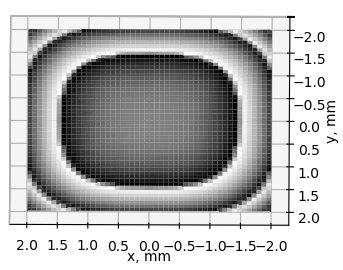
\includegraphics[width=10cm]{plots/aievenphase_new}
            \caption{Двумерная фаза модифицированного входного поля Эйри при $\alpha  = 3$}
            \label{aieven_phase_2d}
        \end{center}
    \end{figure}

    Нетрудно заметить общую схожесть получившейся картины с ранее продемонстрированной фазой входного поля пучков Пирси.
    Таким образом, на данном этапе уже можно высказать предположение,
    что общий вид выходной картины модифицированного пучка структурно будет повторять внешний вид пучка Пирси.

    Аналогичные рассуждения справделивы и для пучков Пирси.
    В данном случае ставится обратная задача -- приведение четной функции в показателе экспоненты к нечетному аналогу,
    однако такого же элегантного решения проблемы нет, а наиболее удобной реализацией станет кусочно-заданная функция следующего вида:
    \[PeOdd(x) = \left\{
    \begin{array}{lr}
        \exp(i(x^4 + tx^2)) & : x \ge 0\\
        \exp(i(-x^4 - tx^2)) & : x < 0
    \end{array}
    \right.
    \]
    Тогда внешний вид входного распределения для двумерного модифицированного пучка Пирси примет вид, приведенный на рисунке~\ref{peodd_phase_2d}.
    \begin{figure}[H]
        \begin{center}
            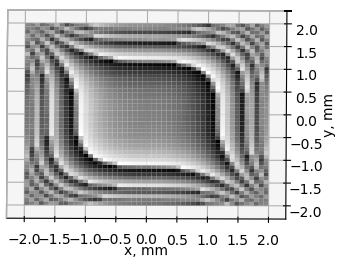
\includegraphics[width=10cm]{plots/peoddphase_new}
            \caption{Двумерная фаза модифицированного входного поля Эйри при $\alpha  = 1$}
            \label{peodd_phase_2d}
        \end{center}
    \end{figure}
    В данном случае также достигнут желаемый результат: картина входного поля модифицированного пучка схожа с входным распределением стандартного пучка Эйри.
    В дальнейшем будет произведено сравнение результатов моделирования пар схожих пучков для оценки степени их подобия.
    \sloppy{
    \tab Подробная реализация программного модуля, осуществляющего построение входного распределения модифицированных пучков и
    визуализацию отдельных их параметров, представлена в разделе 1 приложения А.
    }
    }\label{subsec:изменение-характеристик-пространственных-спектров}
    }\label{sec:построение-входных-распределений-пучков-эйри,-пирси-и-их-модификаций-в-виде-пространственных-спектров}
    \newpage


    \section{\nohyphens{Моделирование формирования пучков с помощью преобразования Фурье}}{
    Основной прием, который можно использовать при моделировании
    формирования пучков с помощью линзы – это перебор различных параметров:
    некоторые из них будут обусловлены физическими характеристиками линзы, а
    некоторые – особенностями методов создания пучков.

    Кроме того, поскольку в рамках данной работы был реализован метод
    численного интегрирования, имеется возможность варьировать размер и отрезок покрытия
    входного и выходного массивов аргументов. Массив аргументов выходной
    функции будет оказывать не такое сильное влияние на общую картину, тогда
    как увеличение размерности и уменьшение интервала между отсчетами массива
    аргументов входной функции будет в значительно большей степени оказывать
    влияние на эксперимент. Это объясняется тем, что для подсчета конечного
    количества значений выходного поля требуется усечь область, на которой
    рассматривается входное поле со всей вещественной оси до какого-то отрезка.
    При таком подходе преобразование Фурье от исходной функции будет
    представлять из себя свертку исходного вида преобразования Фурье с
    функцией sinc:
    \begin{align*}
        \int^{c_2}_{c_1} Ai(x)exp[-ixt]dx &= \frac{c_2-c_1}{2\pi}\int^{\infty}_{-\infty}exp[\frac{ix^3}{3} + \frac{i(c_1+c_2)}{2}(x-t)] \times\\
        & \times sinc[\frac{c_2-c_1}{2}(x-t)]dx,
    \end{align*}
    которая при увеличении рассматриваемого отрезка до всей
    вещественной оси обратится в дельта-импульс, вернув преобразованию Фурье
    исходный вид. Из этого можно сделать вывод, что влияние функции $sinc$ на
    точность преобразования будет ослабевать по мере увеличения отрезка
    рассмотрения входного поля~[\ref{Khonina_2011}].

    Программная реализация функции численного интегрирования,
    выполняющей преобразование Фурье представлена в разделе 2 приложения А. Логика
    работы программы такова, что функция интегрирования одинаково
    работает со всеми видами входных полей, так что его использование для
    моделирования распространения пучков конкретного вида требует только
    указания искомой функции в качестве параметра метода.

    Как уже было сказано ранее, физический смысл преобразования Фурье -- распространение пучка через линзу.
    Приведем условную схему оптической установки, соответствующей данному физическому процессу.
    Ее внешний вид представлен на рисунке~\ref{four_sys}.
    \begin{figure}[H]
        \begin{center}
            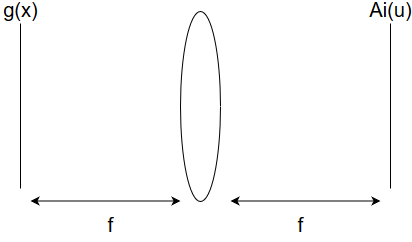
\includegraphics[width=10cm]{plots/four_sys}
            \caption{Схема оптической установки для распространения пучка через линзу}
            \label{four_sys}
        \end{center}
    \end{figure}

    На данной схеме видны две плоскости: входная, находящаяся слева от линзы, и выходная,
    находящаяся с противоположной стороны. Обе плоскости находятся на фокусном расстоянии $f$ от линзы,
    то есть являются фокальными. На входной плоскости начинает свое распространение входная функция пучка,
    а на выходной плоскости формируется результат моделирования -- сформированный пучок.

    На следующих рисунках представлены результаты моделирования
    формирования пучков Эйри и Пирси с различными параметрами. Для
    краткости воспользуемся следующими обозначениями: $x$ – массив аргументов
    входной функции, представляющий собой набор равноудаленных друг от друга
    элементов на вещественной оси абсцисс на участке от левой до правой
    границы, $u$ – массив аргументов выходной функции, представляющий собой
    набор равноудаленных друг от друга элементов на вещественной оси абсцисс
    на участке от левой до правой границы, $\alpha$ – значение параметра функции
    входного поля.

    Результат моделирования пучка Эйри представлен на рисунке~\ref{airyoutput}.
    \begin{figure}[H]
        \begin{center}
            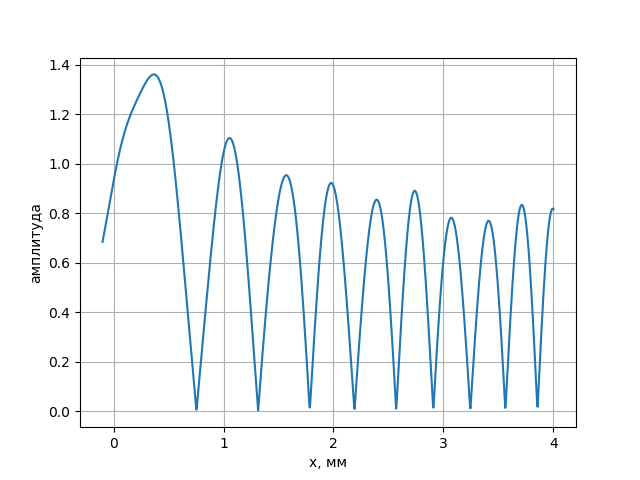
\includegraphics[width=10cm]{plots/airyoutput}
            \caption{Амплитуда выходного поля пучков Эйри, $x \in [-2; 2],  \alpha  = 10$}
            \label{airyoutput}
        \end{center}

    \end{figure}

    Как уже было сказано выше, одной из целей, преследуемых в данной работе,
    является выявление влияния различных параметров на выходную картину.
    Рассмотрим поочередно сравнение выходных картин при изменении фокусного расстояния линзы,
    параметра входной функции и входного отрезка рассмотрения. Результаты моделирования приведены на рисунках \ref{ai_focus_comparison} - \ref{ai_input_comparison}.

    \begin{figure}[H]
        \begin{center}
            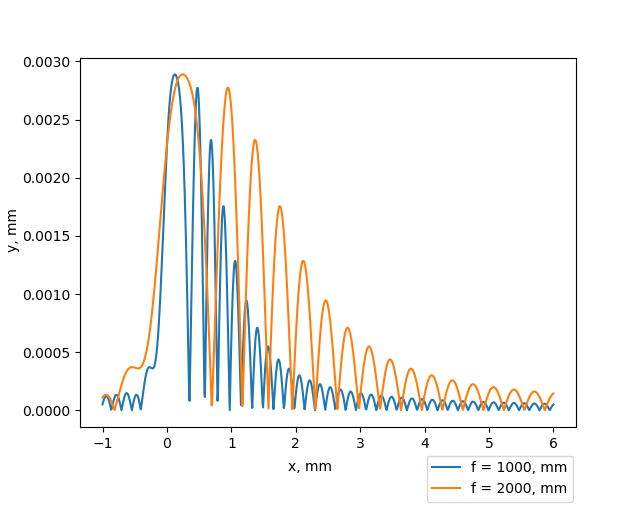
\includegraphics[width=10cm]{plots/ai_focus_comparison}
            \caption{Сравнение пучков Эйри для различных фокусных расстояний}
            \label{ai_focus_comparison}
        \end{center}
    \end{figure}

    \begin{figure}[H]
        \begin{center}
            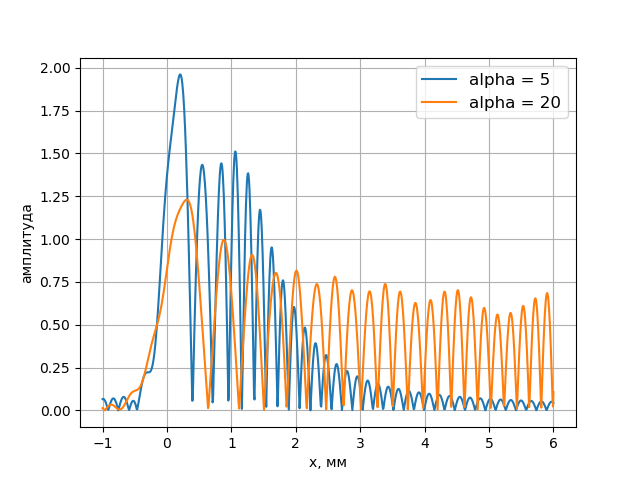
\includegraphics[width=10cm]{plots/ai_param_comparison}
            \caption{Сравнение пучков Эйри, полученных для различных параметров входной функции}
            \label{ai_param_comparison}
        \end{center}
    \end{figure}

    \begin{figure}[H]
        \begin{center}
            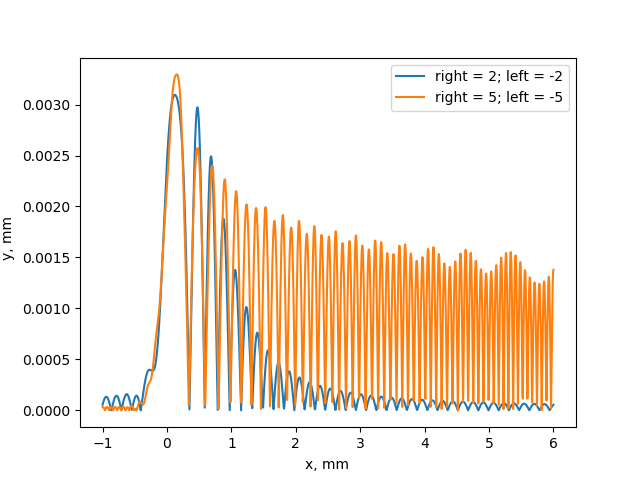
\includegraphics[width=10cm]{plots/ai_input_comparison}
            \caption{Сравнение пучков Эйри для различных входных отрезков}
            \label{ai_input_comparison}
        \end{center}

    \end{figure}

    Ранее в данной работе было предположено, что увеличение параметра входной функции приведет к похожему результату,
    который можно получить с помощью увеличения отрезка рассмотрения.
    Теперь можно утверждать, что данное предположение было верно, поскольку можно наблюдать,
    насколько существенно увеличилось потенциальное расстояние распространения,
    как при увеличении входного отрезка, так и при увеличении параметра входной функции.
    Увеличение фокусного расстояния линзы дает привычный и понятный эффект,
    который можно назвать масштбаированием, то есть визуально он воспринимается как приближение картинки,
    чему и соответствует увеличение фокусного расстояния линзы, например, в фотоаппарате.

    Стоит отметить, что в теории амплитуда выходного поля
    равномерно затухает, так что волнообразность максимумов графиков на
    рисунках~\ref{ai_param_comparison} -~\ref{ai_input_comparison} является дефектом,
    который неизбежно возникнет при моделировании или физической реализации. Как уже было сказано выше, это
    объясняется необходимостью сужения до конечного отрезка области
    рассмотрения входной функции.

    Проведем исследование влияния различных параметров на ширину пучка, то есть на расстояние
    от первого пика до последнего перед окончательным затуханием пучка.

    Для исследования первой зависимости для конкретного измерения зафиксируем фокусное расстояние и входной размер
    и будем изменять параметр $\alpha$. Результат эксперимента представлен в следующей таблице.\\
    \begin{table}[H]
	\centering
	\caption{ Зависимость ширины графика от параметра \alpha }
	\begin{tabularx}{0.9\textwidth}{ | Y | Y  | Y | Y |Y |}
		\hline
		$\alpha_1$ & $\alpha_2$ & $dist_1,$ мм & $dist_2,$ мм & $\frac{dist_2}{dist_1}$ \\ \hline
		15 & 30 & 0.9 & 1.9 & 2.2 \\ \hline
		20 & 30 & 1.2 & 1.9 & 1.6\\ \hline
        20 & 40 & 1.2 & 2.7 & 2.2\\ \hline
        15 & 45 & 0.9 & 3.0 & 3.4\\ \hline
	\end{tabularx}
	\label{tab1}
    \end{table}

    Из данных в таблице можно сделать вывод о том, что увеличение параметра действительно положительно
    влияет на ширину пучка, и что наблюдается практически линейная зависимость между отношениями параметров
    и максимальной шириной графиков, соответствующих этим параметрам.

    Поступим аналогичным образом и исследуем влияение фокусного расстояния на максимальную ширину пучка.
    Данные, полученные в ходе исследования, представлены в следующей таблице.\\

    \begin{table}[H]
        \caption{ Зависимость ширины графика от фокусного расстояния }
	\centering

	\begin{tabularx}{0.9\textwidth}{ | Y | Y  | Y | Y |Y |}
		\hline
		$f_1,$ мм & $f_2,$ мм & $dist_1,$ мм & $dist_2,$ мм & $\frac{dist_2}{dist_1}$ \\ \hline
		150 & 300 & 1.5 & 3.0 & 2.0 \\ \hline
		200 & 400 & 2.0 & 4 & 2.0\\ \hline
        200 & 600 & 2 & 5.9 & 1.9\\ \hline
        300 & 450 & 0.8 & 1.2 & 1.5\\ \hline
	\end{tabularx}
	\label{tab2}
    \end{table}

    Можно наблюдать, что увеличение фокусного расстояния также положительно влияет на ширину графика и отношение фокусных расстояний практически
    полностью совпадает с отношением ширин графиков пучков.

    Проведем последнее сравнение, в котором будем варьировать входной размер при зафиксированных других параметрах.
    Будем рассматривать симметричные входные размеры, поэтому приведем в таблице только правую его границу.
    Результаты эксперимента представлены в следующей таблице.\\

\begin{table}[H]
	\centering
	\caption{ Зависимость ширины графика от входного размера }
	\begin{tabularx}{0.9\textwidth}{ | Y | Y  | Y | Y |Y |}
		\hline
		$x_1,$ мм & $x_2,$ мм & $dist_1,$ мм & $dist_2,$ мм & $\frac{dist_2}{dist_1}$ \\ \hline
		1 & 2 & 0.2 & 0.7 &  3.7\\ \hline
		1 & 3 & 0.2 & 1.6 & 8.0\\ \hline
        2 & 3 & 0.7 & 1.6 & 2.3\\ \hline
        2.6 & 4 & 3.5 & 9.1 & 2.5\\ \hline
        2 & 4 & 0.7 & 3.0 & 4.2\\ \hline
	\end{tabularx}
	\label{tab3}
    \end{table}

    Из последнего сравнения нельзя сделать однозначного вывода о характере зависимости входного размера и ширины графика,
    однако можно заметить, что данная зависимость близка к квадратичной.

    Проведем аналогичные сравнения для пучков Пирси. Результат моделирования формирования пучка Пирси представлен на рисунке~\ref{pearceyoutput3},
    а сравнение различных реализаций при изменении параметров на рисунках~\ref{pe_focus_comparison} -~\ref{pe_input_comparison}.

    \begin{figure}[H]
        \begin{center}
            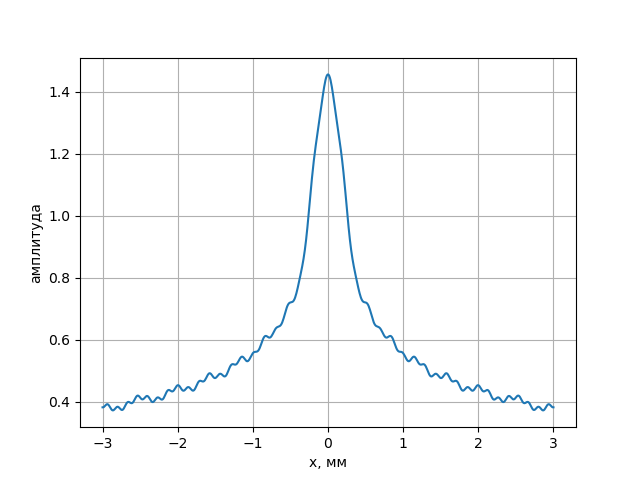
\includegraphics[width=10cm]{plots/pearceyoutput3}
            \caption{Амплитуда выходного поля пучков Пирси при $ \alpha  = 1, f = 1000$}
            \label{pearceyoutput3}
        \end{center}
    \end{figure}

    \begin{figure}[H]
        \begin{center}
            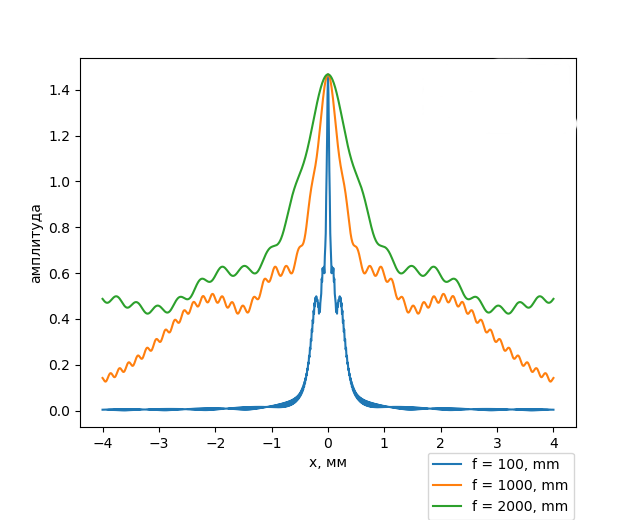
\includegraphics[width=10cm]{plots/pe_focus_comparison}
            \caption{Сравнение пучков Пирси для различных фокусных расстояний}
            \label{pe_focus_comparison}
        \end{center}
    \end{figure}

    \begin{figure}[H]
        \begin{center}
            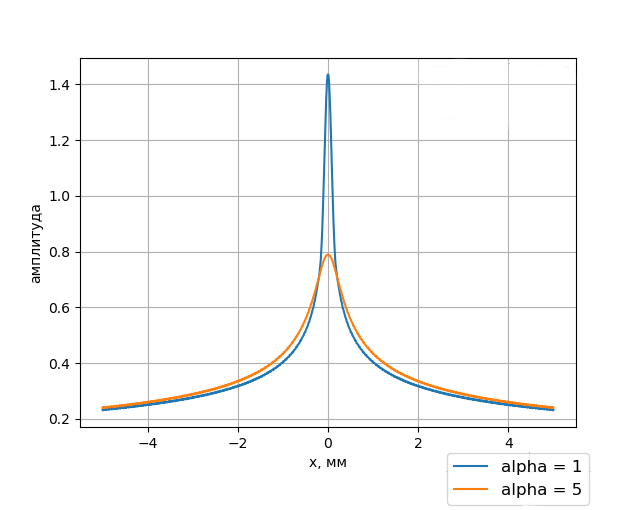
\includegraphics[width=10cm]{plots/pe_param_comparison}
            \caption{Сравнение пучков Пирси, полученных для различных параметров входной функции}
            \label{pe_param_comparison}
        \end{center}
    \end{figure}

    \begin{figure}[H]
        \begin{center}
            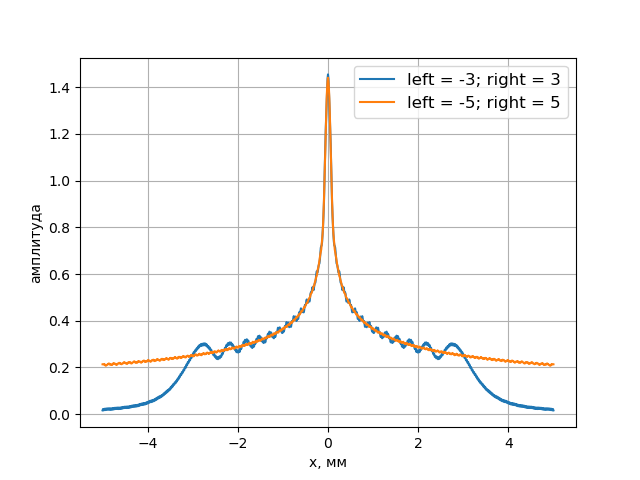
\includegraphics[width=10cm]{plots/pe_input_comparison}
            \caption{Сравнение пучков Пирси для различных входных отрезков}
            \label{pe_input_comparison}
        \end{center}
    \end{figure}

    Общий ход рассуждений при описании сравнений пучков Пирси с различными
    параметрами идентичен рассуждениям относительно пучков Эйри.
    Cтоит только отметить, что колебания на ветвях графиков объясняются эффектом Гиббса
    из-за ограниченной апертуры оптической установки [\ref{gibbs}].

    Далее рассмотрим изменения в картине амплитуды выходного поля при
    изменении параметра входного поля и фокусного расстоянии линзы f на
    примере пучков Пирси с зафиксированными параметрами $x \in [-1; 2], u \in [-3; 3]$.
    Сравнивая графики на рисунках~\ref{pearceyoutput} и~\ref{pearceyoutput1}, можно увидеть, какое влияние
    оказывает несимметричность массива аргументов входной функции
    относительно отрезка рассмотрения выходной функции.

    \begin{figure}[H]
        \begin{center}
            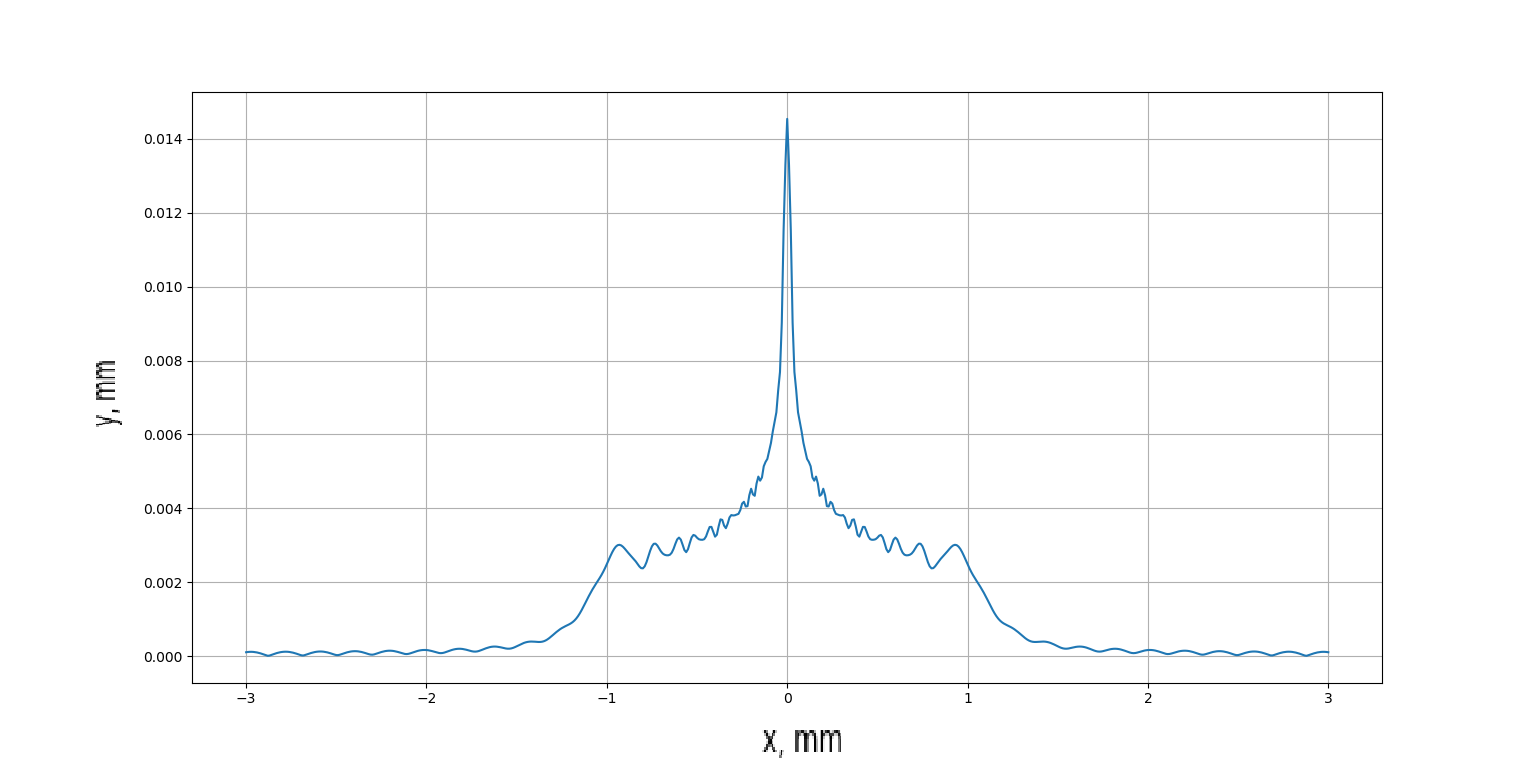
\includegraphics[width=10cm]{plots/pearceyoutput}
            \caption{Амплитуда выходного поля пучков Пирси, $x \in [-3; 3], \alpha  = 1$}
            \label{pearceyoutput}
        \end{center}

    \end{figure}

    \begin{figure}[H]
        \begin{center}
            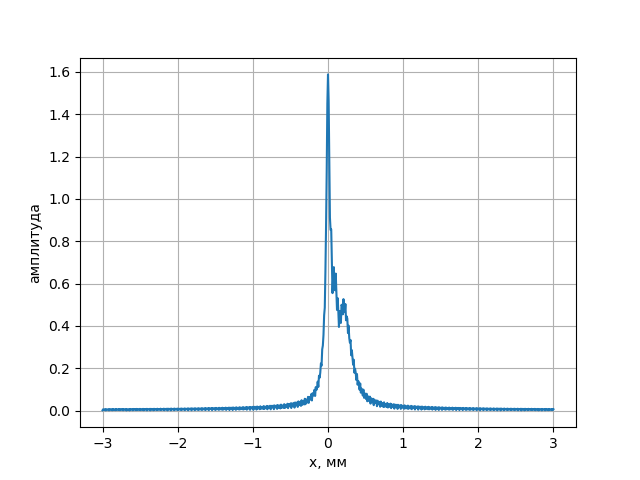
\includegraphics[width=10cm]{plots/pearceyoutput1}
            \caption{Амплитуда выходного поля пучков Пирси, $x \in [-1; 2], \alpha  = 1$}
            \label{pearceyoutput1}
        \end{center}

    \end{figure}


    Можно легко убедиться в корректности результатов, сравнив полученные
    изображения с готовыми результатами, опубликованными в научных статьях по
    этой теме~[\ref{airy_acc}].

    Попробуем убедиться в том, что модификации, произведенные над пучками в предыдущем разделе,
    действительно привели к желаемому результату и изменили их свойства ожидаемым образом.
    Для начала подвергнем рассмотрению модифицированный пучок Эйри,
    функция в показателе экспоненты у которого теперь стала четной функцией.
    Результат моделирования представлен на рисунке \ref{aieven_output}.
    \begin{figure}[H]
        \begin{center}
            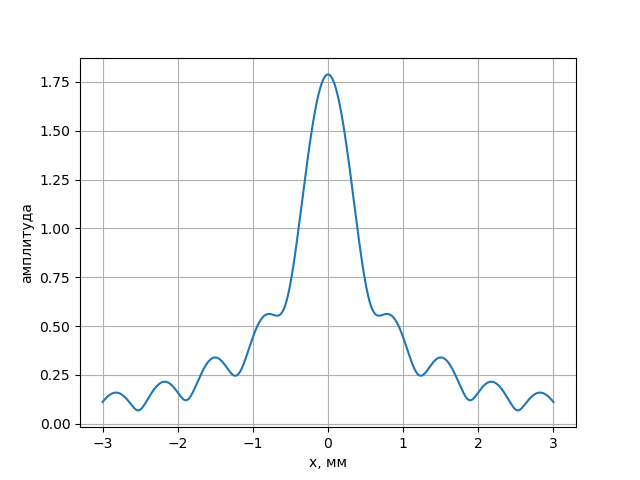
\includegraphics[width=10cm]{plots/aieven_output}
            \caption{Амплитуда выходного поля модифицированного пучка Эйри, $ \alpha  = 5, f = 2000$}
            \label{aieven_output}
        \end{center}
    \end{figure}
    Нетрудно заметить схожесть графика на последнем рисунке с, например,
    рисунком~\ref{pearceyoutput3}. Данная схожесть наблюдается для разных фокусных расстояний и параметров,
    однако в этом нет ничего удивительного, так как фактически входные функции пучков остаются разными,
    хотя и имеют ряд одинаковых свойств.

    Несколько интереснее ситуация обстоит во втором случае, когда модифицировался пучок Пирси,
    так как из нашего предположения следует, что новая реализация должна была получить некоторые новые свойства,
    в частности, свойство ускорения. Рассмотрим результат моделирования, представленный на рисунке \ref{peodd_output}.
    \begin{figure}[H]
        \begin{center}
            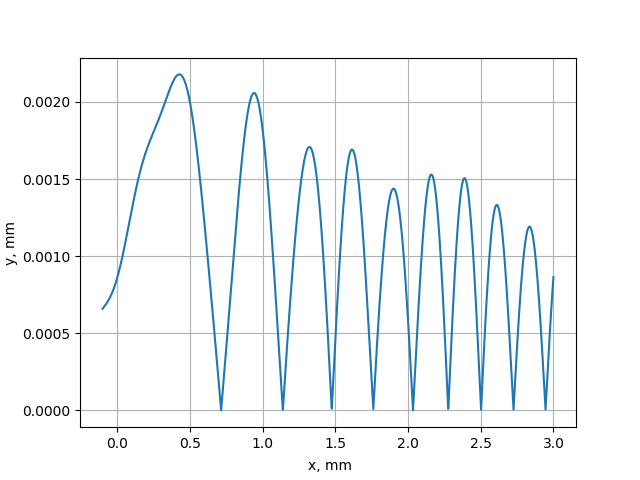
\includegraphics[width=10cm]{plots/peodd_output}
            \caption{Амплитуда выходного поля модифицированного пучка Пирси, $ \alpha  = 5, f = 2000$}
            \label{peodd_output}
        \end{center}
    \end{figure}
    Очевидно сходство рисунка~\ref{peodd_output} с рисунком~\ref{airyoutput}, однако хотелось бы убедиться в том,
    что, кроме внешнего сходства, подобные преобразования передают некоторые свойства пучков.
    Проверка этой гипотезы осуществляется в разделе 6.
    }\label{sec:nohyphens}
    \newpage

    \section[Моделирование распространения пучков с помощью преобразования Френеля]{\nohyphens{Моделирование распространения пучков с помощью преобразования Френеля}}{

    Рассмотрим результаты, полученные в ходе применения к рассматриваемым пространственным спектрам оператора
    распространения на произвольное расстояние. В целом, существенных отличий преобразования Френеля от Фурье не так много,
    а кроме того, преобразование Френеля связано с преобразованием Фурье и может быть представлено через через него,
    однако данный факт выходит за рамки исследования данной научной работы.
    Как уже объяснялось ранее, в теории бесконечные пучки Пирси и Эйри являются бездифракционными,
    однако на практике нам приходится обрезать отрезки рассмотрения или моделирования.
    В таком случае пучки остаются бездифракционными только на определенном расстоянии.
    Этим объясняется изменение внешнего вида пучков при увеличении расстояния распространения.
    Стоит отметить, что прохождение луча через линзу по своей сути ускоряет его свободное распространение,
    поэтому сформировать пучки Эйри или Пирси можно не только с помощью описанного ранее преобразования Фурье,
    но и с помощью распространения входного луча на достаточно большое расстояние.

    Алгоритм вычисления значения интеграла в заданной точке представлен на рисунке~\ref{listing}.
    \begin{figure}[H]
        \begin{center}
            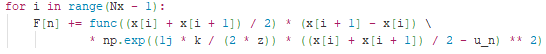
\includegraphics[width=10cm]{plots/listing}
            \caption{Фрагмент кода, отвечающий за вычисление значения интеграла в заданной точке}
            \label{listing}
        \end{center}
    \end{figure}

    Приведем общий вид оптической схемы, выполняющей преобразование Френеля, на рисунке~\ref{fres_sys}.
    \begin{figure}[H]
        \begin{center}
            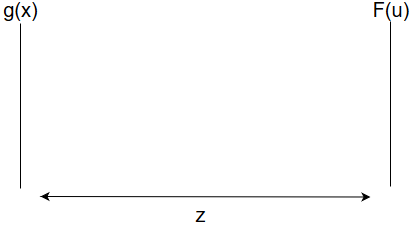
\includegraphics[width=10cm]{plots/fres_sys}
            \caption{Схема оптической установки для свободного распространения луча}
            \label{fres_sys}
        \end{center}
    \end{figure}

    Общий вид преобразования Френеля \eqref{fresnel}, как и основные принципы перехода к формулам численного интегрирования \eqref{integration},
    уже были описаны в работе, так что перейдем к рассмотрению полученных результатов,
    представленных на рисунках~\ref{fres300} -~\ref{fres1200}.

    \begin{figure}[H]
        \centering
        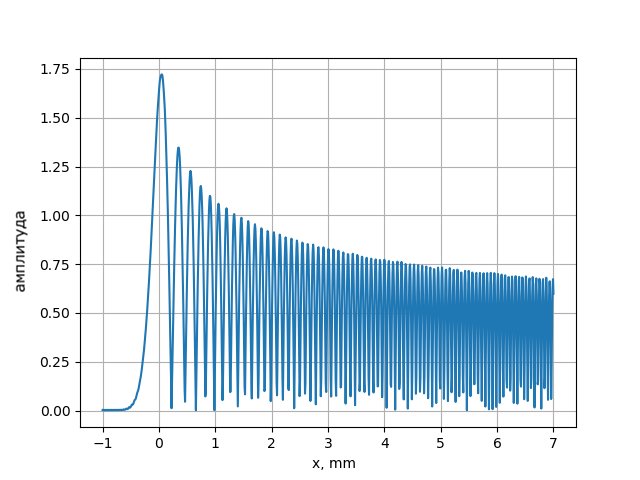
\includegraphics[height = 9cm]{plots/fres300.png}
        \caption{График амплитуды пучка Эйри при $z = 300$мм}
        \label{fres300}
    \end{figure}

    \begin{figure}[H]
        \centering
        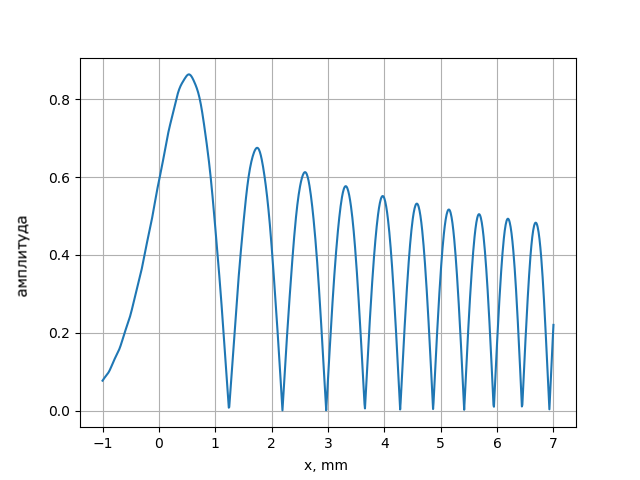
\includegraphics[height = 10cm]{plots/fres1200.png}
        \caption{График амплитуды пучка Эйри $z = 1200$мм}
        \label{fres1200}
    \end{figure}
    \vspace{0.5cm}
    Подробное описание реализации программного модуля, осуществляющего преобразование Френеля, приведено в разделе 3 приложения А.

    }\label{sec:nohyphens2}

    \newpage
    \section[Моделирование распространения пучка вблизи фокальной области]{\nohyphens{Моделирование распространения пучка вблизи фокальной области}}{
    В процессе моделирования может возникнуть интерес к случаю,
    который не описывается приведенными выше операторами распространения.
    Например, может возникнуть необходимость распространять уже сформированный пучок на некоторое расстояние вблизи фокальной области.
    Нетрудно догадаться, что в сути своей реализация данного случая требует
    совмещения физического смысла преобразований Фурье и Френеля.
    Рассмотрим этот случай подробнее.

    Для реализзации данного случая существуют две опции:
    \begin{enumerate}[\arabic*)]
        \item включение оптического элемента в оператор распространения на свободное расстояние;
        \item распространение пучка, полученного при прохождении входной функции через линзу.
    \end{enumerate}
    \vspace{0.2cm}
    Как уже было описано в разделе теоретических сведений,
    преобразование Френеля справедливо только для расстояний распространения много
    больше размеров входного окна. Второй способ не требует проведения никаких
    дополнительных математических преобразований, однако он не снимает ограничения на расстояние распространения,
    то есть с его помощью будет проблематично получить картину в ближней зоне.
    Первый способ в свою очередь позволяет в некоторой степени этим ограничением пренебречь,
    однако требует проведения дополнительных математических преобразований,
    которые делают это возможным. Дополним для этого преобразование Френеля~\eqref{fresnel} следующим оптическим элементом:
    \begin{equation*}
        exp[-ik \frac{x^2}{2f} ].
    \end{equation*}

    Тогда раскроем квадрат в показателе экспоненты, вынесем за знак интеграла слагаемое, содержащее $u^2$,
    так как оно не зависит от переменной интегрирования,
    и внесем добавленный оптический элемент под знак интеграла.
    После группировки некоторых слагаемых получим:
    \begin{equation*}
        F(u) = - \sqrt{\frac{ik}{2 \pi z}}exp[ikz] exp[{ \frac{iku^2}{2z} }] \int_{-\infty}^{+\infty}f(x) exp[\frac{ikx^2}{2}( \frac{1}{z} - \frac{1}{f})] exp[{ik \frac{ux}{z}}]dx,
    \end{equation*}
    \tab где $f$ -- фокусное расстояние линзы;\\
    \tab \tab \hspace{-0.4cm}$z$ -- расстояние от начальной плоскости до линзы.


    По физическому смыслу оба случая идентичны, так что оптические схемы будут для них одинаковыми,
    хотя стоит отметить, что первый случай позволяет получить картину и до фокусного расстояния линзы,
    в то время как использование второго способа дает возможность увидеть картину только после его прохождение через линзу.

    Однако не стоит забывать, что при использовании второго варианта в процессе вычислений
    входные данные дважды подвергаются усеканию, что не может не отразиться на качестве
    выходной картины и допустимых областях рассмотрения. Иными словами после формирования пучка
    дальнейшему распространению подвергается только та его часть, которая попала в выходное окно для преобразования Фурье,
    так что, вообще говоря, рассматривать существенно большее выходное окно для дальнейшего преобразования Френеля возможно,
    но практически не имеет смысла. Учтем данный факт при дальнейшем моделировании.

    Вид оптической схемы, осуществляющей оба описанных преобразования, представлен на рисунке~\ref{four_fres_sys}.

    \begin{figure}[H]
        \begin{center}
            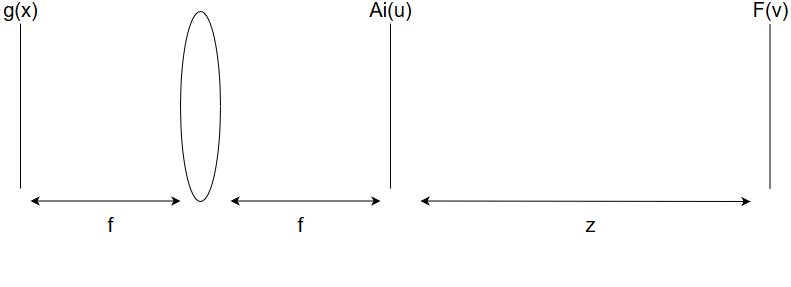
\includegraphics[width=10cm]{plots/four_fres_sys}
            \caption{Схема оптической установки для свободного распространения пучка, сформированного с помощью линзы}
            \label{four_fres_sys}
        \end{center}
    \end{figure}
    Данная схема не нуждается в подробном описании, поскольку является последовательным объединением схем,
    изображенных на рисунках~\ref{four_sys} и~\ref{fres_sys}, описанных ранее.

    Реализация интегрирования в данной функции аналогична предыдущим реализациям.
    Также стоит заметить, что для данного случая справедливо замечание
    о получения двумерного преобразования из одномерного в частных случаях.

    Поскольку две опции, обозначенные в начале раздела, несколько разделили сферы собственного применения,
    то приведем оба результата. Результаты моделирования, полученные с помощью второго способа,
    будут выглядеть аналогично иллюстрациям из предыдущего раздела. Первый способ тоже подходит для этой цели,
    однако это отличный инструмент, чтобы продемонстрировать свойство ускорения, которое присуще некоторым видам пучков.
    В данной работе данным свойством обладают пучки Эйри и, по выдвинутому предположению,
    модификация пучка Пирси, при котором его входная функция становится нечетной функцией.
    Свойство ускорения будет наблюдаться в ближней зоне, то есть при формировании пучка в точке близкой к точке начала распространения.

    Продемонстрируем результат моделирования с помощью второго способа на рисунке~\ref{four_fres_300_400}.
    Нетрудно увидеть существенное сходство с полученными ранее результатами, например,~\ref{fres300}.
    \begin{figure}[H]
        \centering
        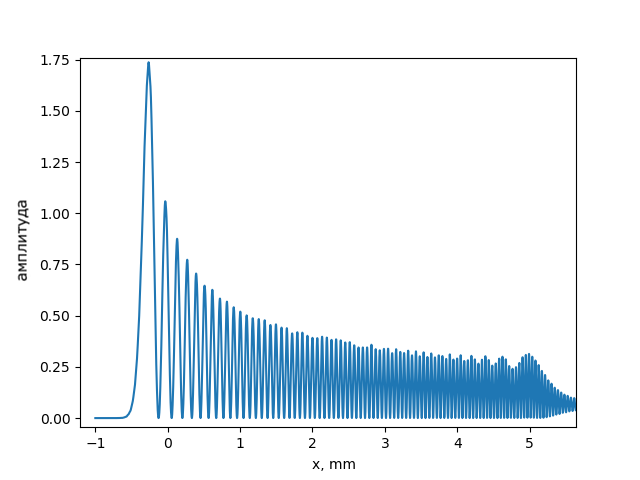
\includegraphics[height = 10cm]{plots/four_fres_300_400.png}
        \caption{График амплитуды пучка Эйри при $f = 300$мм, $z = 400$мм}
        \label{four_fres_300_400}
    \end{figure}
    \vspace{0.5cm}

    Перейдем теперь к рассмотрению свойства ускорения, которое легко можно получить с помощью первого способа.
    Для этого зафиксируем начальную и конечную точки рассмотрения и пройдемся по получившемуся отрезку с зафиксированным шагом,
    вычисляя на каждой итерации полученное преобразование для заданного расстояния.
    Результатом данного вычислительного эксперимента станут изображения рисунках~\ref{correct_acc} -~\ref{correct_acc_peodd}.
    \begin{figure}[H]
        \centering
        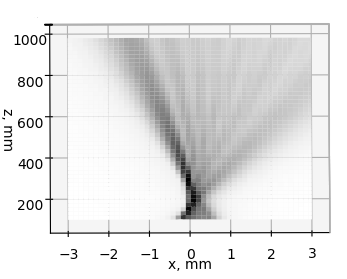
\includegraphics[height = 10cm]{plots/ai_acc_before_focus.png}
        \caption{Ускорение пучка Эйри, $f = 100$, мм}
        \label{correct_acc}
    \end{figure}

    \begin{figure}[H]
        \centering
        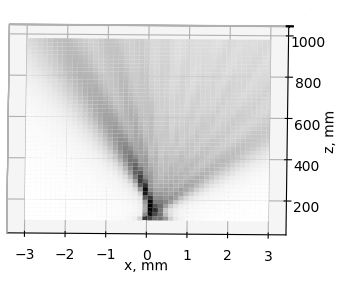
\includegraphics[height = 10cm]{plots/pe_acc_before_focus.png}
        \caption{Ускорение нечетного пучка Пирси, $f = 100$, мм}
        \label{correct_acc_peodd}
    \end{figure}
    \vspace{0.4cm}
    В данной цветовой карте темные темные области находятся выше светлых областей.
    В таком случае на рисунке~\ref{correct_acc_peodd} зависимость отклонения наиболее ярко
    выраженного пика от расстояния распространения отлична от линейной.
    Именно это явление и называется ускорением, и в данном эксперименте было подтверждено наличие свойства ускорения
    у модифицированного пучка Пирси, что также находит подтверждение в [\ref{first_airy}].
    Кроме того, можно заметить, что наиболее узкая и четкая область изображения соответствует приблизительному
    фокусному расстоянию линзы, что отвечает общеизвестным принципам работы собирающей линзы.

    Оценим влияние рассмотренных ранее параметров на величину ускорения, а именно их влияние на смещение главного пика относительно начала отсчета координат.
    Для этого поочередено зафиксируем два параметра и расстояние, изменяя
    при этом третий. Для первого эксперимента будем изменять параметр \alpha. Расстояние распространение зафиксировано на значении 400мм. Результаты приведены в следующей таблице.\\

    \captionsetup[table]{name={Таблица},labelsep=endash,singlelinecheck=false, skip=5pt, margin=1cm}

    \begin{table}[H]
        \caption{ зависимость смещение от параметра  \alpha}
	\centering

	\begin{tabularx}{0.9\textwidth}{ | Y | Y  |}
		\hline
		$\alpha,$ мм  & $offset$ \\ \hline
		5 & 0.5 \\ \hline
		10 & 0.4 \\ \hline
        20 & 0.3 \\ \hline
        40 & 0.1\\ \hline
        80 & 0 \\ \hline
	\end{tabularx}
	\label{tab4}
    \end{table}

    Как видно из данных в таблице, увеличение параметра \alpha негативно влияет на ускорение пучка. Для следующего эксперимента будем изменять фокусное расстояние
    при зафиксированных остальных параметрах. Результаты приведены в следующей таблице.\\
    \begin{table}[H]
	\centering
	\caption{ Зависимость смещения от фокусного расстояния }
	\begin{tabularx}{0.9\textwidth}{ | Y | Y  |}
		\hline
		$f,$ мм  & $offset$ \\ \hline
		100 & 1.2 \\ \hline
		150& 0.6 \\ \hline
        200 & 0.3 \\ \hline
        250 & 0.1 \\ \hline
        300 & 0 \\ \hline
	\end{tabularx}
	\label{tab5}
    \end{table}

    Данные из таблицы указывают на то, что величина фокусного расстояния приблизительно обратно пропорциональна смещению главного пика.
    Кроме того, измерения показали, что при фокусном расстоянии $f \geq 300$ явление ускорения практически полностью перестает
    наблюдаться вне зависимости от величины остальных параметров.

    Для последнего эксперимента сравним смещение в зависимости от величины входного размера. Поскольку рассматриваются только симметричные участки, в таблице будет приведена только
    правая граница размера. Результаты представлены в следующей таблице.\\
    \begin{table}[H]
	\centering
	\caption{ Зависимость смещения от входного размера }
	\begin{tabularx}{0.9\textwidth}{ | Y | Y  |}
		\hline
		Правая граница, мм  & Смещение, мм  \\ \hline
		1 & 0.30 \\ \hline
        1.5 & 0.27 \\ \hline
		2 & 0.27 \\ \hline
        2.5 & 0.26 \\ \hline
        3 & 0.26 \\ \hline

	\end{tabularx}
	\label{tab6}
    \end{table}

    Как видно из данных, приведенных в таблице, увеличение входного размера несколько снижает смещение, однако
    можно утверждать, что это влияние не столь сущесвтенно.

    Попробуем также установить, для какого из рассмотренных ускоряющихся пучков величина ускорения больше.
    Для этого зададим обоим пучкам одинаковые параметры \alpha, фокусные расстояния и входные размеры и посмотрим,
    каким образом изменяется величина отклонения при увеличении расстояния распространения.\\

    \begin{table}[H]
	\centering
	\caption{ Сравнение смещений пучков}
	\begin{tabularx}{0.9\textwidth}{ | Y | Y  | Y  |}
		\hline
		Расстояние, мм  & Смещение Эйри, мм  & Смещение нечетного Пирси, мм\\ \hline
		100 & -0.11 & 0.02 \\ \hline
        150 & 0.00 & 0.10\\ \hline
		200 & -0.02 & 0.15\\ \hline
        250 & -0.17 & 0.16\\ \hline
        300 & -0.30 & 0.13\\ \hline
        350 & -0.45 & 0.06\\ \hline
        400 & -0.60 & 0.01\\ \hline
	\end{tabularx}
	\label{tab7}
    \end{table}

    Как видно из таблицы, ускорения пучка Эйри существенно больше, чем у пучка Пирси.
    Исходя из того факта, что было установлено, что увеличение параметра \alpha негативно влияет на величину ускорения,
    можно попытаться объяснить это явление тем, что во входной Функции Эйри множитель \alpha делится на 3, так что при одних и тех же параметрах
    величина параметра оказывает разное влияение на пучок Эйри и модифицированный пучок Пирси.

    Таким образом, за исключением минорных отличий, была продемонстрирована возможность модификации пучков Эйри и
    Пирси в аналогичные друг другу с приобретением свойств желаемого пучка.

    Подробное описание модуля, реализующего совмещение преобразований Френеля и Фурье, приведено в разделе 4 приложения А.

    }
    \newpage
    \section{Формирование двумерных пучков}{
    В общем виде двумерное преобразование Фурье уже было описано равенством~\eqref{2d_four}.

    Аналогично прежним рассуждениям, для вычисления двумерного преобразования Фурье использовалось численное
    интегрирование методом прямоугольников. Полная реализация преобразования приведена в приложении.

    Нетрудно заметить, что вычислительная сложность используемого алгоритма составляет $O(n^4)$,
    если мы рассматриваем одинаковые квадратные входные и выходные области.
    Для получения удовлетворительный точности результатов время выполнения программы может
    превышать несколько минут. В связи с этим стоит заметить, что в частном случае,
    когда входная и выходная области симметричны, двумерное преобразование Фурье может
    быть получено из одномерного с помощью факторизации. Это осуществимо за счет разделимости подынтегрального
    выражения на два идентичных, каждое из которых зависит только от одной переменной.
    Данный метод позволяет существенно сократить время вычислений даже для моделирования с большей точностью,
    однако применим только в частном случае, например, он не будет подходить в случае
    намеренного зануления некоторых участков входного распределения.

    На рисунках~\ref{pe3d} -~\ref{ai3d} приведены результаты моделирования двумерного преобразования Фурье.
    \begin{figure}[H]
        \centering
        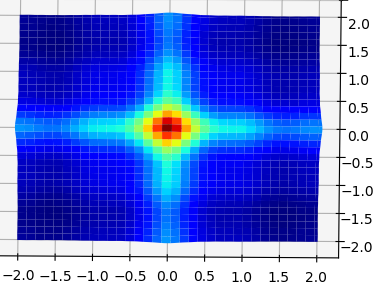
\includegraphics[height = 10cm]{plots/pe3d}
        \vspace{0.2cm}
        \caption{График амплитуды двумерного пучка Пирси при $f = 650$мм}
        \label{pe3d}
    \end{figure}

    \vspace{0.6cm}

    \begin{figure}[H]
        \centering
        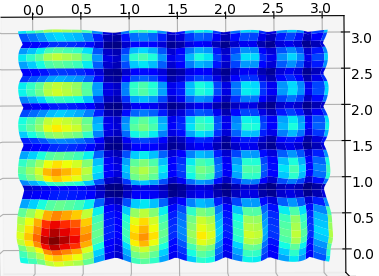
\includegraphics[height = 10cm]{plots/ai3d}
        \vspace{0.4cm}
        \caption{График амплитуды двумерного пучка Эйри при $f = 650$мм}
        \label{ai3d}
    \end{figure}
    }\label{sec:моделирование-трехмерной-картины-распространения-пучков}


    \newpage
    \titleformat{\section}{\bfseries\centering}{\thesection}{0.5em}{\MakeUppercase}

    \section*{Заключение}
    {
    \addcontentsline{toc}{section}{Заключение}
    В рамках данной работы были реализованы
    программные модули построения входных распределений в виде пространственных спектров пучков Эйри и Пирси, моделирования
    формирования пучков при прохождении через линзы и распространении на свободное расстояние, а также через оптическую систему,
    позволяющую моделировать распространение пучков вблизи фокальной области. Можно отметить, что
    результаты работы программы соответствуют действительности, так как
    совпадают с результатами, представленными в статьях, посвященных
    рассмотрению проблем аналогичной тематики, которые использовались в
    качестве библиографических источников. Также в пользу корректности результатов говорит дублирование некоторых результатов,
    полученных различными способами. В ходе выполнения работы были
    установлены некоторые закономерности между значениями параметров
    входных полей и операторов распространения и общим видом выходного поля. Было установлено, что
    увеличение объема входных данных положительно сказывается на общем виде
    выходной картины и расстоянии потенциального распространения, что достигается за счет увеличения отрезка рассмотрения
    входной функции, а также увеличения параметра входной функции. Было
    отмечено, что увеличение фокусного расстояния линзы при моделировании
    распространения пучков масштабирует график, что соответствует привычному принципу работы собирающей линзы.

    Над пучками были проведены модификации с целью выявить возможность приобретения рассматриваемыми
    пучками некоторых свойств, характерных для пучков, чей внешний вид был взят в качестве желаемого
    результата для модификаций. Данное предположение нашло подтверждение:
    в частности, модифицированный пучок Пирси стал обладать свойством ускорения,
    чего нельзя сказать о его классическом виде.

    Без внесения конструктивных изменений использование разработанной
    программы можно распространить на большое семейство пучков, что может
    являться объектом исследования в дальнейших работах. Кроме того, объектом исследования
    может стать свойство недифрагированности пучков, как представляющее существенный интерес
    современной науки. Реализованный модуль
    действительно можно использовать для моделирования и анализа
    распространения пучков перед переходом к физической реализации оптической
    установки.

    \newpage
    }



    %------------------------------------------------
    % Список литературы
    %------------------------------------------------
    \section*{Список использованных источников}{
    \def\bibindent{-1cm}
    \renewcommand\refname{Список использованных источников}
    \addcontentsline{toc}{section}{Список использованных источников}

    \begin{enumerate}[label=\arabic*]
        \urlstyle{rm}

        \item \sloppy{
        Siviloglou, G.A. Observation of Accelerating Airy Beams [Текст] / G. A.
        Siviloglou [and other] // Physical Review Letters. -- 2007. -- Vol. 99(21), 213901. \label{first_airy} }

        \item \sloppy{
        Airy beam [Электронный ресурс] // Википедия : свободная энцикл. –
        Электрон. дан. – [Б. м.], 2018. – URL: \url{https://en.wikipedia.org/wiki/Airy_beam} (дата обращения: 11.11.2018). \label{airy_wiki}}


        \item \sloppy{
        Catastrophe theory [Электронный ресурс] // Википедия : свободная
        энцикл. – Электрон. дан. – [Б. м.], 2018. – URL:  \url{https://en.wikipedia.org/wiki/Catastrophe_theory}
        (дата обращения: 10.12.2018). \label{catastrophe}}



        \item \sloppy{
        Хонина, С. Н. Ограниченные одномерные пучки Эйри: лазерный веер
        [Текст] / С.Н. Хонина, С.Г. Волотовский // Компьютерная оптика. – 2008 – Т.
        32, № 2. – С.168-174. \label{Khonina_2008}}

        \item \sloppy{
        Auto-focusing and self-healing of Pearcey beams [Текст]
        / James D. Ring [and others] // Optics express -- 2012 -- Vol. 20, № 17. -- P. 18955-18966. \label{pe_selfheal}}


        \item \sloppy{
        Khonina, S. N. Specular and vortical Airy beams [Текст] / Svetlana N.
        Khonina // Optics Communications – 2011 – № 284(19) – P. 4263–4271 \label{Khonina_2011}}

        \item \sloppy{
        M. Abramowitz Handbook of Mathematical Functions [Текст] / M.
        Abramowitz, I.A. Stegun. – Dover, 1972. – 456 p. \label{math_func}}

         \item\sloppy{
        Зорич В. А. Математический анализ [Текст]/ Зорич В. А. — М.: Физматлит, 1984. — 544 с.\label{zorich} }



        \item \sloppy{
        Virtual source of a Pearcey beam [Текст] / Dongmei Deng [and others] // Optics Letters. – 2014. –
        T. 39, № 9. – P. 2703-2706 \label{pe_art}}

        \item \sloppy{
        Самарский А.А. Численные методы  [Текст] /
        Самарский А.А., Гулин А.В. — М.: Наука. Гл. ред. физ-мат. лит., 1989.— 432 с. \label{samarsky}}

       \item \sloppy{ Залманзон Л.A. Преобразования Фурье, Уолша, Хаара и их применение в управлении, связи и других областях [Текст]/
        Залманзон Л.A. — М.: Наука. Гл. ред. физ.-мат. лит., 1989. - 496 с. \label{fres} }

        \item \sloppy{
        Numpy and Scipy Documentation [Электронный ресурс] // Официальный
        сайт документации библиотек Numpy и Scipy – Электрон. дан. – 2018 URL:
        \url{https://docs.scipy.org/doc/} (дата обращения: 11.11.2018) \label{np}}

        \item \sloppy{
        Mathematical functions for complex numbers [Электронный
        ресурс] // Документация: стандартная библиотека Python – Электрон. дан. – 2018. – URL: \url{https://docs.python.org/2/library/cmath.html} (дата обращения:
        14.11.2018) \label{cmath}}
         \vspace{-0.9cm}
        \item \sloppy{
        Matplotlib Documentation [Электронный ресурс] // Официальный сайт
        библиотеки Matplotlib – Электрон. дан. – 2018. -- URL:
        https://matplotlib.org/3.0.2/index.html (дата обращения: 15.11.2018) \label{plt}}

        \item \sloppy{
        Gibbs phenomenon [Электронный ресурс] // Википедия : свободная энцикл. –
        Электрон. дан. – [Б. м.], 2019. – URL: \url{https://en.wikipedia.org/wiki/Gibbs_phenomenon} (дата обращения: 25.5.2019) \label{gibbs}}

        \item \sloppy{
        Acelerating optical beams [Текст] / Miguel A. Bandres [and others]  // Optics and photonics news – 2013 – Vol. 24(6) –
        P. 30-37 \label{airy_acc}}

%        \item\sloppy{
%        Fresnel diffraction [Электронный ресурс] // Википедия : свободная энцикл. –
%        Электрон. дан. – [Б. м.], 2019. – URL: \url{https://en.wikipedia.org/wiki/Fresnel_diffraction} (дата обращения:
%        17.2.2019) \label{fres} }



    \end{enumerate}
    }

%    \begin{thebibliography}{20\kern\bibindent}
%        \setlength{\itemindent}{1cm}
%        \urlstyle{rm}
%
%        \bibitem{first_airy}
%        Siviloglou, G.A. Observation of Accelerating Airy Beams [Текст] / G. A.
%        Siviloglou [and other] // Physical Review Letters. -- 2007. -- Vol. 99(21), 213901.
%
%        \bibitem{airy_wiki}
%        Airy beam [Электронный ресурс] // Википедия : свободная энцикл. –
%        Электрон. дан. – [Б. м.], 2018. – URL: \url{https://en.wikipedia.org/wiki/Airy_beam} (дата обращения: 11.11.2018).
%
%
%        \bibitem{catastrophe}
%        Catastrophe theory [Электронный ресурс] // Википедия : свободная
%        энцикл. – Электрон. дан. – [Б. м.], 2018. – URL:  \url{https://en.wikipedia.org/wiki/Catastrophe_theory}  (дата обращения: 10.12.2018).
%
%
%
%        \bibitem{Khonina_2008}  Хонина, С. Н. Ограниченные одномерные пучки Эйри: лазерный веер
%        [Текст] / С.Н. Хонина, С.Г. Волотовский // Компьютерная оптика. – 2008 – Т.
%        32, № 2. – С.168-174.
%
%        \bibitem{pe_selfheal} Auto-focusing and self-healing of Pearcey beams [Текст] / James D. Ring [and others] // Optics express -- 2012 -- Vol. 20, № 17. -- P. 18955-18966.
%
%
%        \bibitem{Khonina_2011}
%        Khonina, S. N. Specular and vortical Airy beams [Текст] / Svetlana N.
%        Khonina // Optics Communications – 2011 – № 284(19) – P. 4263–4271
%
%        \bibitem{math_func}
%        M. Abramowitz Handbook of Mathematical Functions [Текст] / M.
%        Abramowitz, I.A. Stegun. – Dover, 1972. – 456 p.
%
%        \bibitem{pe_art}
%        Virtual source of a Pearcey beam [Текст] / Dongmei Deng [and others] // Optics Letters. – 2014. –
%        T. 39, № 9. – P. 2703-2706
%
%        \bibitem{samarsky}  Самарский А.А. Численные методы  [Текст] / Самарский А.А., Гулин А.В. — М.: Наука. Гл. ред. физ-мат. лит., 1989.— 432 с.
%
%        \bibitem{np}
%        Numpy and Scipy Documentation [Электронный ресурс] // Официальный
%        сайт документации библиотек Numpy и Scipy – Электрон. дан. – 2018 URL:
%        \url{https://docs.scipy.org/doc/} (дата обращения: 11.11.2018)
%
%        \bibitem{cmath}
%        Mathematical functions for complex numbers [Электронный
%        ресурс] // Документация: стандартная библиотека Python – Электрон. дан. – 2018. – URL: \url{https://docs.python.org/2/library/cmath.html} (дата обращения:
%        14.11.2018)
%
%        \bibitem{plt}
%        Matplotlib Documentation [Электронный ресурс] // Официальный сайт
%        библиотеки Matplotlib – Электрон. дан. – 2018. -- URL:
%        https://matplotlib.org/3.0.2/index.html (дата обращения: 15.11.2018)
%
%
%
%        \bibitem{gibbs}
%        Gibbs phenomenon [Электронный ресурс] // Википедия : свободная энцикл. –
%        Электрон. дан. – [Б. м.], 2019. – URL: \url{https://en.wikipedia.org/wiki/Gibbs_phenomenon} (дата обращения: 25.5.2019)
%
%        \bibitem{airy_acc}
%        Acelerating optical beams [Текст] / Miguel A. Bandres [and others]  // Optics and photonics news – 2013 – Vol. 24(6) –
%        P. 30-37
%
%        \bibitem{fres}
%        Fresnel diffraction [Электронный ресурс] // Википедия : свободная энцикл. –
%        Электрон. дан. – [Б. м.], 2019. – URL: \url{https://en.wikipedia.org/wiki/Fresnel_diffraction} (дата обращения:
%        17.2.2019)
%
%
%    \end{thebibliography}


    \newpage

    %------------------------------------------------
    % Приложения. Коды программ и.т.д.
    %------------------------------------------------
    \titleformat{\subsection}[block]{\sloppy \bfseries \hspace{1.2cm} }{\thesubsection}{0.5em}{}
    \setlength{\droptitle}{-1cm}
    \lstset{
    identifierstyle=\ttfamily,
    keywordstyle=\ttfamily,
     showspaces=false, showstringspaces=false,
    breaklines = false
    }
    \section*{Приложение А}
    {
    \addcontentsline{toc}{section}{Приложение А Код программы}
    \begin{center}
        \textbf{Код программы}
    \end{center}

    \subsection*{\nohyphens{А.1 Модуль, отвечающий за входное распределение пучков }}{
    \addcontentsline{toc}{subsection}{А.1 Модуль, отвечающий за входное распределение пучков}
    \lstinputlisting[language=python,mathescape=true]{sources/beams_report.py}

    }

    \subsection*{\nohyphens{ А.2 Модуль, отвечающий за применение преобразования Фурье к данным }}{
    \addcontentsline{toc}{subsection}{А.2 Модуль, отвечающий за применение преобразования Фурье к данным}
    \lstinputlisting[language=python,mathescape=true]{sources/fourier_report.py}
    }

    \subsection*{\nohyphens{А.3 Модуль, отвечающий за применение преобразования Френеля к данным }}{
    \addcontentsline{toc}{subsection}{А.3 Модуль, отвечающий за применение преобразования Френеля к данным}
    \lstinputlisting[language=python,mathescape=true]{sources/fresnel_report.py}
    }

    \subsection*{\nohyphens{А.4 Модуль, содержащий в себе вспомогательные функции для моделирования и построения}}{
    \addcontentsline{toc}{subsection}{А.4 Модуль, содержащий в себе вспомогательные функции для моделирования и построения}
    \lstinputlisting[language=python,mathescape=true]{sources/utils_report.py}
    }


    }

\end{document}
